% !TeX document-id = {ca28df42-0773-4265-bb7c-b21d86ed4d82}
%%%%%%%%%%%%%%%%%%%%%%%%%%%%%%%%%%%%%%%%%%%%%%%%%
%
%	MSc THESIS TEMPLATE
%	developed for my master thesis at the Universitá di Torino
%
%	by Eugenio Senes (eugenio.senes@gmail.com)
%
%	released under MIT license, so share, modify and enjoy, but quoting the author !
%
%%%%%%%%%%%%%%%%%%%%%%%%%%%%%%%%%%%%%%%%%%%%%%%%%

%% DOCUMENT CLASS (alternative to book is 'report')
% Print just right page or both sides (comment the other one)
\documentclass[12pt,a4paper,openright,oneside]{book}	%%One sided
%\documentclass[12pt,a4paper,openright,twoside]{book}	%%Double sided
\newcommand{\singlenodegraph}[1]{
  \tikz{\node [rounded corners, scale=0.9, draw, fill=gray!30, font=\footnotesize] {#1}}
}
%% SET MARGINS OF THE PAGES
\usepackage{geometry}
\geometry{a4paper,portrait, left=35mm, right=20mm, top=35mm, bottom=30mm}

%% HEADERS AND FOOTERS
\usepackage{fancyhdr}
\pagestyle{fancy}
\fancyhf{} 			%clears default header and footer
\rhead{} 			%right head
\lhead{ \leftmark} 	%left head
\rfoot{\thepage}
%%consider using also chead, cfoot, lfoot
%coherce the plain stile to this (e.g. the first page of every chapter)
\fancypagestyle{plain}{
	\fancyhf{}
	\rfoot{\thepage}
	\renewcommand{\headrulewidth}{0pt}
	\renewcommand{\footrulewidth}{0pt}
}
%% CLEAR PAGE WITHOUT NUMBER AT THE BEGINNING OF CHAPTERS
\let\origdoublepage\cleardoublepage
\newcommand{\clearemptydoublepage}{%
  \clearpage
  {\pagestyle{empty}\origdoublepage}%
}
%% ALLOW PAGE ROTATION
\usepackage{lscape}
\usepackage[english, italian]{babel} %%Set Italian as main language of the document
%% HYPERTEXT SETUP
\usepackage{hyperref}
\usepackage{ragged2e}
\usepackage{enumerate}

%% redefinition of /autoref naming conventions to italian names
\addto\extrasitalian{
	\def\figureautorefname{Figura}
	\def\equationautorefname{Equazione}
}
\hypersetup{
    colorlinks,
    citecolor=black,
    filecolor=black,
    linkcolor=black,
    urlcolor=black
}
%% PDF SETTINGS
\hypersetup{
    pdfauthor={Andrea Zito, Emanuele Rovaretto, Lorenzo Bafunno},
    pdftitle={shortTitle},
    pdfsubject={subject},
    pdfkeywords={Semantic Web, Type Systems, Haskell, OCaml}
}
%% FONTS AND SYMBOLS
\usepackage[utf8]{inputenc}	%%input font setting
\usepackage[T1]{fontenc} 		%%font for automatic recognition of letters with the accent
\usepackage{amsfonts}		%%fonts for the mathematical rendering of formulas
\usepackage{amssymb}
\usepackage{amsmath}
\usepackage{amsthm}
\usepackage{thmtools}
\usepackage{syntax}

\newtheorem{definition}{Definizione}
%% CHAPTERS STRUCTURE

%% FIGURES
\usepackage{graphicx}
\usepackage{subfigure}		%%allow side by side figures with single caption
%% TABLES
\usepackage{multirow}		%%allow to merge rows in the tables
\usepackage{booktabs}		%%allow use of \toprule, \midrule, \bottomrule in tables
%%CAPTIONS
\usepackage{caption}
%% BIBLIOGRAPHY
\usepackage[babel]{csquotes}
%% CODE LISTINGS
\usepackage{listings}		%%allow to use code listings

\usepackage{tikz}
\usepackage{prooftree}
\usepackage{minted}
\usemintedstyle{perldoc}
\usetikzlibrary{positioning,
                quotes}

%% HYPENATON
\hyphenation{te-si pip-po paperino}	%manual hyphenation

%%%%%%%%%%%%%%%%%%%%%%%%%%%%%%%%%%%%%%%%%%%%%%%%%
%%%% BEGIN DOCUMENT
\begin{document}

%%%%%% HEAD  OF THE DOCUMENT
\frontmatter
%%FRONT PAGE
%\begin{titlepage}
    %upper part

    %logo
    \begin{center}
        
\includegraphics[scale=.3]{head/logo.png}
    \end{center}
    %title
    \begin{center}
        \vspace{20mm}
        {{\Large{\textsc{\bf Universit\`a degli Studi di Torino \\} \vspace{2mm} \emph{Corso di Laurea in Informatica}}}}
        \vspace{5mm}
    \end{center}
    \begin{center}
        \vspace{5mm}
        {\LARGE{\bf THE FANCY TITLE\\ OF MY FANCY THESIS\\}}
        \vspace{3mm}
        {\large{Tesi di Laurea\\}}
        %\vspace{5mm}
        %{\LARGE{\bf SECOND ROW TITLE}}
    \end{center}
    \vspace{20mm}
    %relatore
    \par
    \noindent
    \begin{minipage}[t]{0.47\textwidth}
        {\large{\bf Relatore/Relatrice:\\}}
        {\large{
                Bono Viviana
            }}
        \vspace{8mm}
        {\large{\bf \\ Controrelatore:\\
                Prof.\\
                Zio Paperone}}
    \end{minipage}
    \\
    \null\hfill
    \begin{minipage}[t]{0.40\textwidth}
        \vspace{20mm}
        {\large{\bf Candidato:\\
                Lorenzo Bafunno\\
            } \large{Matricola 944233}}
    \end{minipage}
    \vspace{10mm}
    \begin{center}
        {\large{Anno Accademico 2022/2023}}
    \end{center}

\end{titlepage}
\begin{titlepage}
    %upper part

    %logo
    \begin{center}
        
\includegraphics[scale=.3]{head/logo.png}
    \end{center}
    %title
    \begin{center}
        \vspace{20mm}
        {{\Large{\textsc{\bf Universit\`a degli Studi di Torino \\} \vspace{2mm} \emph{Corso di Laurea in Informatica}}}}
        \vspace{5mm}
    \end{center}
    \begin{center}
        \vspace{5mm}
        {\LARGE{\bf THE FANCY TITLE\\ OF MY FANCY THESIS\\}}
        \vspace{3mm}
        {\large{Tesi di Laurea\\}}
        %\vspace{5mm}
        %{\LARGE{\bf SECOND ROW TITLE}}
    \end{center}
    \vspace{20mm}
    %relatore
    \par
    \noindent
    \begin{minipage}[t]{0.47\textwidth}
        {\large{\bf Relatore:}\\
            Bono Viviana}\\
        \vspace{4mm}
        \\
        {\large{\bf Correlatore:}\\
        Lieto Antonio\\
        Marco
        }
        %\vspace{8mm}
        %{\large{\bf \\ Controrelatore:\\
        %Prof.ssa Nonna Papera}}
    \end{minipage}
    \\
    \null\hfill
    \begin{minipage}[t]{0.40\textwidth}
        \vspace{20mm}
        {\large{\bf Candidato:\\
                Lorenzo Bafunno\\
            } \large{Matricola 944233}}
    \end{minipage}
    \vspace{10mm}
    \begin{center}
        {\large{Anno Accademico 2022/2023}}
    \end{center}

\end{titlepage}
\clearemptydoublepage
%%DEDICATION (the initial quote) & statement of originality
\thispagestyle{empty}
\begin{flushright}

    \vspace*{60mm}

    The amazing quote\\
    that I chose as inspiration\\
    for this work\\
    \vspace{4mm}
    Author, \textit{Title}\\




\end{flushright}

\vspace*{110mm}
\noindent
\emph{Dichiaro di essere responsabile del contenuto dell'elaborato che presento al fine del
    conseguimento del titolo, di non avere plagiato in tutto o in parte il lavoro prodotto da
    altri e di aver citato le fonti originali in modo congruente alle normative vigenti in
    materia di plagio e di diritto d'autore. Sono inoltre consapevole che nel caso la mia
    dichiarazione risultasse mendace, potrei incorrere nelle sanzioni previste dalla legge e
    la mia ammissione alla prova finale potrebbe essere negata.}
\clearemptydoublepage
%%ABSTRACT
\chapter*{Abstract}

Lorem ipsum dolor sit amet, consectetur adipiscing elit. Vestibulum nec augue tincidunt, sodales lorem fringilla, venenatis metus. Cras dictum nec urna vitae euismod. Nunc vulputate quam dolor, id convallis augue convallis sit amet. Aliquam nec felis sodales, condimentum massa ac, tincidunt nisi. Vestibulum posuere, lacus tempus facilisis cursus, velit libero mattis diam, vel aliquet magna turpis vitae ligula. Maecenas aliquet nulla at gravida mattis. Morbi vestibulum in ex sed ultricies. Morbi sodales mollis mauris, vitae tincidunt enim hendrerit et. Interdum et malesuada fames ac ante ipsum primis in faucibus. Suspendisse laoreet faucibus massa, quis elementum enim eleifend aliquet. Class aptent taciti sociosqu ad litora torquent per conubia nostra, per inceptos himenaeos. Etiam at tortor vestibulum, dictum augue ut, porta lorem. Sed venenatis feugiat diam. Integer eu diam nec dolor viverra hendrerit.

Vestibulum quis vehicula massa. Etiam dictum, enim vel luctus accumsan, dolor velit laoreet metus, nec pretium arcu dui nec nulla. Donec ac sollicitudin justo, ut ullamcorper nunc. Curabitur ornare, ipsum hendrerit dictum rutrum, nisl lectus cursus sapien, in condimentum ipsum magna vel lorem. Cras vulputate semper placerat. In nec quam condimentum, auctor nisl eu, viverra libero. Maecenas scelerisque, odio vel accumsan luctus, justo dui pharetra orci, sit amet feugiat lorem lacus ac enim. Donec ultrices nulla semper erat consectetur, vitae mattis nulla dictum. Fusce maximus tristique condimentum. Quisque et sodales lectus, vel posuere leo. In ac augue vel neque sagittis volutpat at nec justo. Proin bibendum lobortis neque, vitae vulputate lorem viverra in. Etiam neque risus, pretium sed tempor a, pharetra quis arcu. Morbi purus nibh, efficitur nec sollicitudin non, commodo vel massa.

Pellentesque eu neque lacus. Vivamus finibus consectetur tellus id imperdiet. In ut dolor ligula. Vivamus ac vehicula erat. Duis semper lacinia eros, sed ultrices orci tristique at. Proin in pellentesque massa. Nunc ultricies justo eget nibh condimentum sollicitudin. Mauris non ligula eget magna pulvinar pretium vel vitae ante. Aenean lacinia metus vel odio vehicula sollicitudin. Quisque nisi augue, faucibus a nulla faucibus, consequat vehicula elit. Donec dui mi, ornare quis sapien ac, finibus maximus mi. Etiam volutpat, arcu quis posuere sollicitudin, ligula elit tincidunt lectus, non dapibus augue nunc id est. Ut dictum et diam vel vulputate. Aliquam ut nibh eu nibh aliquet aliquam eget ut leo. Duis urna tellus, sodales non ornare ut, aliquet vitae mi. Nunc consequat est vitae elit consectetur, id iaculis libero congue.

Praesent sem neque, semper ac turpis eu, fringilla egestas erat. Fusce in leo velit. Sed faucibus viverra massa. Donec justo lorem, accumsan a nisi in, maximus placerat augue. Mauris posuere aliquet sapien sed viverra. In hac habitasse platea dictumst. Ut nec dictum purus, sit amet gravida risus.

\clearemptydoublepage
%%INDEXES
%summary
\setlength{\headheight}{14.49998pt}
\tableofcontents
\clearemptydoublepage
\chapter{Introduzione}

\section{Scopo della ricerca}
\paragraph{} Questo lavoro è un lavoro di gruppo svolto in collaborazione con Lorenzo Bafunno e Andrea Zito e la consulenza del dottor Marco Antonio Stranisci, della professoressa Rossana Damiano e del professor Antonio Lieto.

L'idea di partenza è stata quella di studiare i benefici dell'applicazione dei linguaggi funzionali e dei sistemi di tipi statici
 rappresentazione della conoscenza. 
 
% ontologie
Le \emph{ontologie} rappresentano un formalismo molto diffuso per la rappresentazione della conoscenza. Un'ontologia si compone di due parti: \emph{T-Box} ( Terminology Box) e \emph{A-Box} (Assertion Box). La prima contiene formule logiche per modellare il dominio, per esempio per affermare che uno 'Studente' è una 'Persona'. La seconda è usata per esprimere asserzioni su individui, per esempio affermare che 'Emanuele' è un istanza di 'Persona'. Un ragionamento su un'ontologia è inferenza di proprietà di interesse, per esempio se si inferisce che 'Persona' ha un nome, allora anche 'Studente' ha un nome, in quanto sua sottoclasse. Le basi di conoscenza rappresentate da ontologie vengono interrogate tramite \emph{query}. Si dice che una query è \emph{abitata} (\emph{inhabited}) se  restituisce dei risultati. Per esempio, una query che cerca le istanze di una 'Pizza Margherita' che allo stesso tempo sia anche un 'Gelato', non è abitata perché potrà mai avere dei risultati, perché nessuna pizza è un gelato (almeno in una base di conoscenza basata sul senso comune).  Una trattazione più avanzata sul tema sarà presentata nel Capitolo \ref{chap:preliminaries}.

% motivazione e obbiettivo
\paragraph{} Dalla nostra indagine (si veda per esempio \cite{baader2017introductionDL}), è emerso che le ontologie non sono più utilizzate nella loro interezza (T-Box e A-Box) perché è troppo dispendioso eseguire ragionamenti formali complessi, anche se così facendo si perde espressività, ignorando una strutturazione più sofisticata dei concetti. Oggigiorno infatti si tende a utilizzare solamente gli A-Box, ovvero le asserzioni sugli individui, per esempio come dati per i modelli basati sul machine learning. Ci siamo quindi chiesti se fosse possibile costruire formalismi che recuperino parte dell'espressività dei ragionamenti formali, senza perdere troppo in efficienza. Una strada che riteniamo promettente è l'uso dei linguaggi funzionali e dei sistemi di tipo per creare applicazioni e nuovi linguaggi che manipolano ontologie spostando i controlli, che di norma vengono compiuti a run-time, a compile-time tramite i sistemi di tipaggio statico.     

\section{Il nostro lavoro}
\paragraph{} Abbiamo cominciato ad analizzare alcuni lavori appartenenti alla letteratura sulla rappresentazione della conoscenza, in particolare sulle ontologie. Abbiamo poi analizzato in dettaglio la tesi di dottorato di Martin Gerhard Leinberger \cite{leinbergerphdthesis}, il quale ha ideato un calcolo con sistema di tipi statico per verificare l'abitabilità delle query SPARQL-CQ trattato nel capitolo \ref{chap:preliminaries}. Noi abbiamo deciso di implementarlo. Bafunno e Zito hanno sottolineato la possibilità di usare un Reasoner (ovvero un sistema in grado di eseguire ragionamenti e deduzioni sulle basi di conoscena) già esistente, indicando HermiT come il più adatto. Per quanto riguarda il linguaggio da utilizzare, assieme a Zito, la prima idea è stata utilizzare Haskell, un linguaggio funzionale che già conoscevamo, ma alla fine la scelta è ricaduta su OCaml (che abbiamo studiato appositamente), un altro linguaggio funzionale più maturo, con più librerie e più interfacciabile con il modulo Reasoner rispetto ad Haskell. 

\paragraph{} Prese queste decisioni architetturali, ho cominciato lo studio per conoscere meglio le due risorse che avrei poi usato nell'implementazione: Hermit \cite{HermiT} e OCaml \footnote{www.ocaml.org}.\\
Ho studiato come utilizzare il reasoner HermiT, compito reso più arduo a causa della poca documentazione presente in rete. Per quanto riguarda OCaml, avendo già un background di Haskell, capire come utilizzarlo non è stato particolarmente impegnativo. \\

\paragraph{} Per l'implementazione, ho deciso di creare due moduli, il modulo Reasoner, scritto in Java, e il modulo OCaml, il primo che performa ragionamenti sull'ontologia, mentre il secondo che implementa il sistema di tipi di Leinberger.

Il mio primo problema è stato far dialogare i due moduli. La soluzione che ho trovato prevede che il modulo OCaml richiami la shell di comando, al quale viene delegata la responsabilità di lanciare il modulo Reasoner.

Un altro grosso problema è stato scegliere la "lingua veicolare" da utilizzare per far comunicare i due moduli: la prima idea è stata quella di definire una grammatica da zero, con tanto di parsificatore da dover usare nel Reasoner: una scelta troppo costosa. Allora ho provato a cercare qualche grammatica già esistente: ho trovato una sintassi sviluppata dall'Università di Manchester per la rappresentazione di ontologie OWL, un particolare tipo di ontologie, con un parsificatore già implementato \footnote{https://ceur-ws.org/Vol-216/submission_9.pdf}. Non rimaneva dunque che adattare il modulo OCaml a quella sintassi e integrare il parsificatore nel modulo Reasoner, per terminare il ponte fra i moduli.

\paragraph{} Il parsificatore e il lexer delle query nel modulo OCaml sono stati facili da realizzare, perché ho usato un generatore di parser e un generatore di lexer per OCaml, OCamlyacc e OCamllex, nei quale mi è bastato specificare la grammatica della query (illustrata nel dettaglio al Capitolo \ref{chap:preliminaries}) e la semantica dei token per ottenere il parsificatore e il lexer. L'unico intoppo l'ho registrato quando ho dovuto cercare di disambiguare la grammatica inizialmente implementata. 

\paragraph{} Il resto dell'implementazione è stato quasi immediato senza grossi problemi, dovendo solo implementare ciò che era già stato progettato da Leinberger.

Attorno al lavoro sull'implementazione del modulo delle query di Leinberger, riassunto sopra nella tesi si trovano:
\begin{itemize}
\item il lavoro di rassegna della letteratura sui tipi e Web Semantico, di cui si è occupato essenzialmente Lorenzo Bafunno (Capitolo \ref{chap:State-of-art});
\item l'implementazione del resto del calcolo di Leinberger, creata principalmente da Andrea Zito (Capitolo \ref{chap:Implementazione});
\item le direzioni di ricerca future, che nascono da riflessioni corali, supportate dal dottor Marco Antonio Stranisci, dalla professoressa Rossana Damiano e dal professor Antonio Lieto (Capitolo \ref{chap:FutureWork}).
\end{itemize}

%%%%%% BODY OF THE DOCUMENT
\mainmatter
%%INTRODUCTION
\chapter{Introduction - How to use this template}

\section{Choose your stile}

Since no style reference has been provided, we are quite free: you have first of all to choose the style and change some lines in the file \url{thesis.tex}. When two options are available, one of the two is commented starting the line with \%. To change it, comment what you don't need and de-comment the other option:

\subsection{Single- or Double-sided}
I like better the Single-sided, but if you want to go double-sided remove at line 14
\begin{verbatim}
\documentclass[12pt,a4paper,openright,oneside]{book}	%%One sided
\end{verbatim}
and de-comment line 15
\begin{verbatim}
\documentclass[12pt,a4paper,openright,twoside]{book}	%%Double sided
\end{verbatim}

\subsection{Headers and footers}
Lines 22-42 are going to use


\subsection{PDF settings}
Insert the information about you and the thesis in lines 56-61. They will be included in the PDF information
\begin{verbatim}
\hypersetup{
    pdfauthor={AuthorName},
    pdftitle={shortTitle},
    pdfsubject={subject},
    pdfkeywords={keyword1, keyword2}
}
\end{verbatim}

\subsection{Language}
The main language is the last, so for a thesis in english line 69 is
\begin{verbatim}
\usepackage[italian,english]{babel} 
\end{verbatim}
Swap ita with eng fi you are writing in italian as main language




\section[Sectioning]{Chapters, sections and subsections}

A thesis has three parts: head, body and tail. Three correspondent folders are containing the source files for these parts.

Any of this source files is imported in the \url{thesis.tex} file, which is the only one to get compiled. This is realised using the command
\begin{verbatim}
\input{subfolder/filename.tex}
\end{verbatim}
To exclude a section from the compiling process, comment or remove the correspondent line. If no subfolder is specified, \LaTeX\ looks for it in the same folder of \url{thesis.tex}

E.g. the introduction source file is in the body subfolder, and is included using the command \begin{verbatim} \chapter{Introduction - How to use this template}

\section{Choose your stile}

Since no style reference has been provided, we are quite free: you have first of all to choose the style and change some lines in the file \url{thesis.tex}. When two options are available, one of the two is commented starting the line with \%. To change it, comment what you don't need and de-comment the other option:

\subsection{Single- or Double-sided}
I like better the Single-sided, but if you want to go double-sided remove at line 14
\begin{verbatim}
\documentclass[12pt,a4paper,openright,oneside]{book}	%%One sided
\end{verbatim}
and de-comment line 15
\begin{verbatim}
\documentclass[12pt,a4paper,openright,twoside]{book}	%%Double sided
\end{verbatim}

\subsection{Headers and footers}
Lines 22-42 are going to use


\subsection{PDF settings}
Insert the information about you and the thesis in lines 56-61. They will be included in the PDF information
\begin{verbatim}
\hypersetup{
    pdfauthor={AuthorName},
    pdftitle={shortTitle},
    pdfsubject={subject},
    pdfkeywords={keyword1, keyword2}
}
\end{verbatim}

\subsection{Language}
The main language is the last, so for a thesis in english line 69 is
\begin{verbatim}
\usepackage[italian,english]{babel} 
\end{verbatim}
Swap ita with eng fi you are writing in italian as main language




\section[Sectioning]{Chapters, sections and subsections}

A thesis has three parts: head, body and tail. Three correspondent folders are containing the source files for these parts.

Any of this source files is imported in the \url{thesis.tex} file, which is the only one to get compiled. This is realised using the command
\begin{verbatim}
\input{subfolder/filename.tex}
\end{verbatim}
To exclude a section from the compiling process, comment or remove the correspondent line. If no subfolder is specified, \LaTeX\ looks for it in the same folder of \url{thesis.tex}

E.g. the introduction source file is in the body subfolder, and is included using the command \begin{verbatim} \chapter{Introduction - How to use this template}

\section{Choose your stile}

Since no style reference has been provided, we are quite free: you have first of all to choose the style and change some lines in the file \url{thesis.tex}. When two options are available, one of the two is commented starting the line with \%. To change it, comment what you don't need and de-comment the other option:

\subsection{Single- or Double-sided}
I like better the Single-sided, but if you want to go double-sided remove at line 14
\begin{verbatim}
\documentclass[12pt,a4paper,openright,oneside]{book}	%%One sided
\end{verbatim}
and de-comment line 15
\begin{verbatim}
\documentclass[12pt,a4paper,openright,twoside]{book}	%%Double sided
\end{verbatim}

\subsection{Headers and footers}
Lines 22-42 are going to use


\subsection{PDF settings}
Insert the information about you and the thesis in lines 56-61. They will be included in the PDF information
\begin{verbatim}
\hypersetup{
    pdfauthor={AuthorName},
    pdftitle={shortTitle},
    pdfsubject={subject},
    pdfkeywords={keyword1, keyword2}
}
\end{verbatim}

\subsection{Language}
The main language is the last, so for a thesis in english line 69 is
\begin{verbatim}
\usepackage[italian,english]{babel} 
\end{verbatim}
Swap ita with eng fi you are writing in italian as main language




\section[Sectioning]{Chapters, sections and subsections}

A thesis has three parts: head, body and tail. Three correspondent folders are containing the source files for these parts.

Any of this source files is imported in the \url{thesis.tex} file, which is the only one to get compiled. This is realised using the command
\begin{verbatim}
\input{subfolder/filename.tex}
\end{verbatim}
To exclude a section from the compiling process, comment or remove the correspondent line. If no subfolder is specified, \LaTeX\ looks for it in the same folder of \url{thesis.tex}

E.g. the introduction source file is in the body subfolder, and is included using the command \begin{verbatim} \input{body/introduction.tex} \end{verbatim}

\subsection{Front page}

Two front pages are provided:
\begin{enumerate}
	\item \url{frontPage.tex} for thesis with a single Relatore
	\item \url{frontPage-cr.tex} for thesis with Relatore and Correlatore
\end{enumerate}
choose what is needed adapting lines 94-95.

\subsection{Dedication}
Dedication is the initial inspirational quote. Can be edited in the file \url{dedication.tex} or removed.

\subsection{Chapter names}
Chapter and section names are in this form:
\begin{verbatim}
\chapter[Name in the index]{Name on the title}
\end{verbatim}
To exclude them from the numbering, use the *; If no name for the index is specified, will be assumed the same. For example:
\begin{verbatim}
\chapter*{Name on the title}
\end{verbatim}
won't be numbered and will have the same name in the title and in the index.

\section{Bulleting}

Bullet list example
\begin{itemize}
	\item first point
	\item second point
	\item third point \\
\end{itemize}

\noindent
Enumeration example
\begin{enumerate}
	\item first point
	\item second point
	\item third point\\
\end{enumerate}

\noindent
Description example
\begin{description}
	\item[first descr] first point
	\item[second descr]  second point
	\item[third descr]  third point\\
\end{description}

\noindent
\dots but you can also build nested lists
\begin{itemize}
	\item first point
	      \begin{itemize} %tab is only for the readability, but not necessary
		      \item first point
		      \item second point
	      \end{itemize}
	\item second point
	\item third point \\
\end{itemize}


\section{Floating objects}

Floating objects are tables, figures and so on.

\subsection{Position, captions and cross-referencing}

To force the position of an object use the options, for example:
\begin{verbatim}
\begin{figure}[htb]
\end{verbatim}
where [htb] means that the priority of positioning is \url{h} = here, \url{t} = top, \url{b} = bottom. Also \url{p} can be used and means that the object is placed in a page on itself.

Captions are managed automatically using the command
\begin{verbatim}
\caption{The title of my object}
\end{verbatim}
to cross reference to the object use the
\begin{verbatim} 
\label{labelName} 
\end{verbatim}
to assign a name to the object and
\begin{verbatim} 
\ref{labelName}
\end{verbatim}
to refer to that.



\subsection{Figures}

Insert a figure using the code
\begin{verbatim} 
\begin{figure}[htb]
\centering

\includegraphics[scale=0.15]{pictures/logo.png}
\caption{the logo of UniTo}
\label{myFigure}
\end{figure}
\end{verbatim}

then you can cross-reference to it. In this case the discussion is about Fig. \ref{myFigure}.

Where the number of the figure has been gotten using
\begin{verbatim} 
\ref{myFigure}
\end{verbatim}


\begin{figure}[htb]
	\centering

	
\includegraphics[scale=0.15]{pictures/logo.png}
	\caption{the logo of UniTo}

\end{figure}

\subsection{Subfigures}

\begin{figure}[htb]
	\centering
	\subfigure[title of first subfigure]
	{
\includegraphics[scale=0.15]{pictures/logo.png}}
	\subfigure[title of second subfigure]
	{
\includegraphics[scale=0.3]{pictures/logo.png}}
	\caption{Two logos of UniTo of different sizes}

\end{figure}

\subsection{Tables}

 \end{verbatim}

\subsection{Front page}

Two front pages are provided:
\begin{enumerate}
	\item \url{frontPage.tex} for thesis with a single Relatore
	\item \url{frontPage-cr.tex} for thesis with Relatore and Correlatore
\end{enumerate}
choose what is needed adapting lines 94-95.

\subsection{Dedication}
Dedication is the initial inspirational quote. Can be edited in the file \url{dedication.tex} or removed.

\subsection{Chapter names}
Chapter and section names are in this form:
\begin{verbatim}
\chapter[Name in the index]{Name on the title}
\end{verbatim}
To exclude them from the numbering, use the *; If no name for the index is specified, will be assumed the same. For example:
\begin{verbatim}
\chapter*{Name on the title}
\end{verbatim}
won't be numbered and will have the same name in the title and in the index.

\section{Bulleting}

Bullet list example
\begin{itemize}
	\item first point
	\item second point
	\item third point \\
\end{itemize}

\noindent
Enumeration example
\begin{enumerate}
	\item first point
	\item second point
	\item third point\\
\end{enumerate}

\noindent
Description example
\begin{description}
	\item[first descr] first point
	\item[second descr]  second point
	\item[third descr]  third point\\
\end{description}

\noindent
\dots but you can also build nested lists
\begin{itemize}
	\item first point
	      \begin{itemize} %tab is only for the readability, but not necessary
		      \item first point
		      \item second point
	      \end{itemize}
	\item second point
	\item third point \\
\end{itemize}


\section{Floating objects}

Floating objects are tables, figures and so on.

\subsection{Position, captions and cross-referencing}

To force the position of an object use the options, for example:
\begin{verbatim}
\begin{figure}[htb]
\end{verbatim}
where [htb] means that the priority of positioning is \url{h} = here, \url{t} = top, \url{b} = bottom. Also \url{p} can be used and means that the object is placed in a page on itself.

Captions are managed automatically using the command
\begin{verbatim}
\caption{The title of my object}
\end{verbatim}
to cross reference to the object use the
\begin{verbatim} 
\label{labelName} 
\end{verbatim}
to assign a name to the object and
\begin{verbatim} 
\ref{labelName}
\end{verbatim}
to refer to that.



\subsection{Figures}

Insert a figure using the code
\begin{verbatim} 
\begin{figure}[htb]
\centering

\includegraphics[scale=0.15]{pictures/logo.png}
\caption{the logo of UniTo}
\label{myFigure}
\end{figure}
\end{verbatim}

then you can cross-reference to it. In this case the discussion is about Fig. \ref{myFigure}.

Where the number of the figure has been gotten using
\begin{verbatim} 
\ref{myFigure}
\end{verbatim}


\begin{figure}[htb]
	\centering

	
\includegraphics[scale=0.15]{pictures/logo.png}
	\caption{the logo of UniTo}

\end{figure}

\subsection{Subfigures}

\begin{figure}[htb]
	\centering
	\subfigure[title of first subfigure]
	{
\includegraphics[scale=0.15]{pictures/logo.png}}
	\subfigure[title of second subfigure]
	{
\includegraphics[scale=0.3]{pictures/logo.png}}
	\caption{Two logos of UniTo of different sizes}

\end{figure}

\subsection{Tables}

 \end{verbatim}

\subsection{Front page}

Two front pages are provided:
\begin{enumerate}
	\item \url{frontPage.tex} for thesis with a single Relatore
	\item \url{frontPage-cr.tex} for thesis with Relatore and Correlatore
\end{enumerate}
choose what is needed adapting lines 94-95.

\subsection{Dedication}
Dedication is the initial inspirational quote. Can be edited in the file \url{dedication.tex} or removed.

\subsection{Chapter names}
Chapter and section names are in this form:
\begin{verbatim}
\chapter[Name in the index]{Name on the title}
\end{verbatim}
To exclude them from the numbering, use the *; If no name for the index is specified, will be assumed the same. For example:
\begin{verbatim}
\chapter*{Name on the title}
\end{verbatim}
won't be numbered and will have the same name in the title and in the index.

\section{Bulleting}

Bullet list example
\begin{itemize}
	\item first point
	\item second point
	\item third point \\
\end{itemize}

\noindent
Enumeration example
\begin{enumerate}
	\item first point
	\item second point
	\item third point\\
\end{enumerate}

\noindent
Description example
\begin{description}
	\item[first descr] first point
	\item[second descr]  second point
	\item[third descr]  third point\\
\end{description}

\noindent
\dots but you can also build nested lists
\begin{itemize}
	\item first point
	      \begin{itemize} %tab is only for the readability, but not necessary
		      \item first point
		      \item second point
	      \end{itemize}
	\item second point
	\item third point \\
\end{itemize}


\section{Floating objects}

Floating objects are tables, figures and so on.

\subsection{Position, captions and cross-referencing}

To force the position of an object use the options, for example:
\begin{verbatim}
\begin{figure}[htb]
\end{verbatim}
where [htb] means that the priority of positioning is \url{h} = here, \url{t} = top, \url{b} = bottom. Also \url{p} can be used and means that the object is placed in a page on itself.

Captions are managed automatically using the command
\begin{verbatim}
\caption{The title of my object}
\end{verbatim}
to cross reference to the object use the
\begin{verbatim} 
\label{labelName} 
\end{verbatim}
to assign a name to the object and
\begin{verbatim} 
\ref{labelName}
\end{verbatim}
to refer to that.



\subsection{Figures}

Insert a figure using the code
\begin{figure}[htb]
\centering

\includegraphics[scale=0.15]{pictures/logo}
\caption{the logo of UniTo}
\label{fig:myfigure}
\end{figure}



then you can cross-reference to it.
In this case the discussion is about Fig\ref{fig:myfigure}

Where the number of the figure has been gotten using
\begin{verbatim} 
\ref{myFigure}
\end{verbatim}


\begin{figure}[htb]
	\centering

	
\includegraphics[scale=0.15]{pictures/logo.png}
	\caption{the logo of UniTo}

\end{figure}

\subsection{Subfigures}

\begin{figure}[htb]
	\centering
	\subfigure[title of first subfigure]
	{
\includegraphics[scale=0.15]{pictures/logo.png}}
	\subfigure[title of second subfigure]
	{
\includegraphics[scale=0.3]{pictures/logo.png}}
	\caption{Two logos of UniTo of different sizes}

\end{figure}

\subsection{Tables}


\clearemptydoublepage
%% CHAPTERS
% add any further chapter file here
\chapter[Concetti preliminari]{Concetti preliminari}\label{chap:preliminaries}
Per poter considerare l'utilizzo dei tipi per il Web Semantico, è necessario analizzare lo stato dell'arte in cui si ritrova questo ambito di ricerca.
Questo capitolo si presta utile per apprendere il vocabolario utilizzato durante tutta la tesi, nonché fornire approfondimenti su nozioni che potrebbero essere date per scontate.
Verranno riassunte le basi dei linguaggi funzionali, così come le componenti del Web Semantico.
\section[Linguaggi funzionali]{Linguaggi funzionali}

\section[Web Semantico]{Web Semantico}
Il World Wide Web è diventato una consolidata rete di conoscenza, che però presenta il difetto che queste informazioni sono pensate per la fruizione umana, piuttosto che da parte di una macchina. Infatti il linguaggio di rappresentazione delle centinaia di pagine che visitiamo ogni giorno, l’HTML, descrive l’impaginazione delle informazioni visualizzate all’utente. Senza un indicazione che spiega il significato dei dati presenti, un agente intelligente non può interpretarne il significato. Uno degli obiettivi del Web Semantico, termine che risale all'articolo del 2001 di Tim-Berners Lee \cite{berners2001semantic}, è cambiare questo paradigma human-centered, permettendo agli agenti artificiali di interpretare e processare la conoscenza presente senza alcun tipo di aiuto umano. È necessario descrivere le informazioni attraverso metadati espressivi, strutturandoli arbitrariamente, che ne spieghino la semantica in un modo che una macchina possa comprenderla.\\
Nel corso degli anni, nella letteratura sono state presentate diverse soluzioni: dagli albori di questo ambito, in cui i dati erano rappresentati in maniera strutturata e formale dalle ontologie, si è giunti alla rappresentazione superficiale ma efficiente del paradigma dei Linked (Open) Data. Questa sezione vuole introdurre agli standard di rappresentazione e recupero dei dati citati in questo lavoro.



\subsection[Resource Description Framework]{Resource Description Framework}
Il Resource Description Framework \cite{RDFspecification} (RDF d'ora in poi) è una serie di specifiche create da W3C (World Wide Web Consortium) che includono un modello per descrivere risorse web attraverso delle annotazioni, sotto forma di \textbf{triple}. Esse consistono in:
\[ < \text{soggetto},\ \text{predicato},\ \text{oggetto} > \]
Un insieme di queste triple, chiamato \textbf{grafo RDF}, può essere rappresentato come un grafo diretto etichettato in cui ogni tripla descrive un arco dal nodo soggetto al nodo oggetto.
\begin{figure}[h]
    \begin{minipage}{0.3\linewidth}
        \centering
        \begin{tikzpicture}[
                node distance = 15mm and 15mm,
                V/.style = {rounded corners, draw, fill=gray!30},
                every edge quotes/.style = {auto, font=\footnotesize, sloped}
            ]
            \begin{scope}[nodes=V]
                \node (1)   {Pizza};
                \node (2) [right=of 1]    {Margherita};
                \node (3) [below =of 2]    {Mozzarella};
                \node (4) [left=of 3]    {Vegetarian};
            \end{scope}
            \draw[->, ultra thick]   (2)  edge["isA"] (1)
            (2)  edge["madeOf"] (3)
            (4)  edge["canEat"] (2);
        \end{tikzpicture}
    \end{minipage}
    \hspace{5mm}
    \begin{minipage}{0.7\linewidth}
        \begin{alignat*}{4}
            G_1 = \{ (\  & \text{Margherita},\  &  & isA,      &  & \text{Pizza}        &  & ),  \\
            (\           & \text{Margherita},\  &  & madeOf,\  &  & \text{Mozzarella}\  &  & ),  \\
            (\           & \text{Vegetarian},\  &  & canEat,\  &  & \text{Mozzarella}\  &  & )\}
        \end{alignat*}
    \end{minipage}
    \caption{un grafo RDF $G_1$ come grafo diretto (sx.) e insieme di triple (dx.)}
    \label{fig:grafoRDF}
\end{figure}

\noindent
Per essere più precisi, \textit{in RDF sia i nodi che i predicati sono risorse}, cioè delle entità nell'universo del discorso d'interesse. A seconda che la risorsa sia una stringa (come Margherita nella \autoref{fig:grafoRDF}) oppure un concetto più astratto è possibile identificarla in due modi diversi: tramite IRI oppure come un letterale. In ogni caso, definire una tripla RDF significa dire che la relazione indicata dal predicato vale fra le risorse indicate dal soggetto e dall'oggetto. Parliamo meglio di questi metodi d'identificazione:
\begin{description}
	\item[IRI (International Resource Identifier)]  Un formato generalizzato di URI che ricorre a un range più ampio di caratteri Unicode, che permette di identificare univocamente una risorsa. È importante sapere che solamente gli IRI vengono utilizzati per identificare i predicati in una tripla, e denotano una \textbf{proprietà}, cioè una risorsa che può essere vista come una relazione binaria.
	Un insieme di IRI destinati all'uso in un grafo RDF è chiamato \textbf{vocabolario RDF} e di solito tutti gli identificatori di uno stesso vocabolario condividono una sotto stringa iniziale comune, che prende il nome di \textbf{namespace}. Per migliorare la leggibilità dei documenti RDF, si utilizza un \textbf{prefisso}, che sostituisce il namespace per abbreviare la lunghezza del identificatore. Ad esempio, per l'IRI \verb|http://example.org/#Margherita| si potrebbe definire il namespace\\ \verb|http://example.org/#| con prefisso \verb|example|; in questo modo la risorsa Margherita può essere identificata con il più corto e leggibile \verb|example:Margherita|. Alcuni esempi concreti possono esseri trovati in \cite{RDFSspecification}.
	\item[Letterali] Rappresentano risorse nel senso di valori numerici, date o stringhe. La codifica di un qualsiasi valore di un letterale è come stringa Unicode, ma è possibile specificare il tipo, identificato da un IRI (e.g. il tipo delle date è \verb|xsd:date|), per permettere di risalire alla vera semantica del valore.
\end{description}
Esiste anche un altro termine che permette di affermare la presenza di un nodo per cui sussiste la relazione, senza nominarlo in maniera esplicita: il \textbf{blank node}. Per fare un paragone, possono essere considerati come variabili esistenziale, in cui il valore non è conosciuto ma si assume che sia presente.

\begin{definition}[Tripla RDF]
	Siano \textbf{I}, \textbf{L} e \textbf{B} rispettivamente gli insiemi infiniti e disgiunti uno a uno delle stringhe IRI, dei letterali e dei blank nodes. Una tripla RDF è una tupla $(s, p, o) \in \textbf{U}\ \cup \textbf{B} \times \textbf{U} \times \textbf{U}\ \cup \textbf{B}\ \cup \textbf{L}.$ in cui s è chiamato soggetto, p il predicato e o l'oggetto.
\end{definition}
\begin{definition}[Grafo RDF]
	Un grafo RDF è un insieme finito di triple RDF.
\end{definition}
\begin{definition}[Grafo RDF]
	Un grafo RDF è un insieme finito di triple RDF.
\end{definition}
IRI (International Resource Identifier),

\subsection{SPARQL CQ}
I grafi RDF vengono interrogati utilizzando le query SPARQL, infatti i grafi vengono memorizzati in database speciali chiamati triplestore, per efficentare le interrogazioni. In questa trattazione utilizziamo un tipo particolare di SPARQL, le query congiuntive, che consistono nella congiunzione di triple pattern, elementi atomici per interrogare un triplestore. \\
\textbf{Abitabilità: } In una query SPARQL, il concetto di abitabilità identifica le query che possono essere abitate da almeno un elemento. Per esempio, se scriviamo una query che richiede tutti i nodi che sono sia di classe Pizza sia di classe Gelato, ovviamente questa query non potrà mai essere abitata, perchè non esistono pizze che allo stesso tempo sono anche dei gelati. Il concetto di abitabilità però non è da confondere con il fatto che essa sia abitata: una query potrebbe essere abitata, ma nel grafo RDF su cui stiamo lavorando non c'è nessun nodo che soddisfa i requisiti. \ 
\begin{figure}[H]
    \centering
    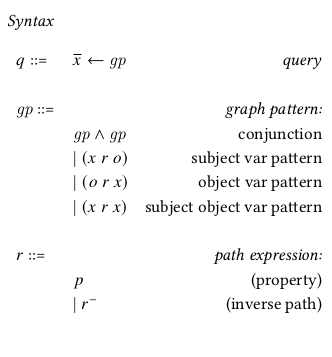
\includegraphics[scale=0.6]{pictures/leinbergSyntax}
    \caption{sintassi delle query \\ SPARQL CQ}
    \label{fig:leinbergerSyntax}
\end{figure}
\newpage
\section[Ontologie]{Ontologie}
La definizione comunemente accettata di ontologia è \textit{una specifica formale ed esplicita di una concettualizzazione condivisa} \cite{goy2015ontologies}. Un modo di rappresentarle è attraverso particolari linguaggi altamente espressivi appartenenti a una famiglia di formalismi chiamati logiche descrittive (DL). Le informazioni sul dominio di interesse vengono espresse in maniera formale tramite formule logiche di due tipologie. Una tipologia fa parte della cosiddetta T-Box e sono asserzioni sulla terminologia, componendo uno schema. L'altra fa parte della A-Box ed è usata per fare asserzioni su individui (astratti), quindi modella le istanze significative. Il T-Box contiene formule logiche (assiomi) che mettono in relazione delle \textit{concept expressions} per modellare il dominio di riferimento, ad esempio il fatto che  uno Student è una Persona. Una \textit{base di conoscenza} è quindi l'insieme di asserzioni presenti sia nel T-Box che nell'A-Box.\\
Nel contesto del Web Semantico, la raccomandazione W3C \textit{Web Ontology Language (OWL)} è una famiglia di linguaggi ontologici altamente espressivi basati sul linguaggio descrittivo $\mathcal{SROIQ}$ \cite{baader2017introductionDL}. Quello che andremo a mostrare noi nella sezione dei costrutti sintattici DL è il più semplice sottoinsieme $\mathcal{ALCOIQ}$.
Grazie alla forma logica delle informazioni, è possibile definire un ragionamento automatico\footnote{\ i.e. tramite un algoritmo deterministico, cioè eseguibile da un computer} che permette di svolgere operazioni di inferenza sugli individui concreti, ad esempio inferire che il nodo \textit{x} di un grafo RDF è uno Studente, ma anche eseguire compiti più astratti, come capire se un concetto è soddisfacibile. Questi compiti sono alla base di ogni reasoner, come ad esempio HermiT \cite{HermiT}, Pellet \cite{Pellet} e Fact++ \cite{Fact++}.\\

\subsection[Logica  descrittiva $\mathcal{ALCOIQ}$]{Logica  descrittiva $\mathcal{ALCOIQ}$}
Questa introduzione e gli esempi sono presi dal libro \cite{baader2017introductionDL}, che contiene un'ottima introduzione alle logiche descrittive. Per non divagare troppo dal motivo per cui spieghiamo questi concetti, ovvero per permettere ai lettori meno esperti delle ontologie di capire la terminologia usata in questa tesi, la logica utilizzata in questa sezione sarà principalmente $\mathcal{ALCOIQ}$. Per questo motivo, useremo anche esempi e tabelle prese dall'introduzione della tesi di dottorato di Leinberger \cite{leinbergerphdthesis}. L'acronimo $\mathcal{ALCOIQ}$ descrive i costrutti sintattici disponibili nel linguaggio (\autoref{fig:SintassiCD}). I costrutti di base sono contenuti in $\mathcal{ALC}$ (\textit{Attributive Language with Complements}), e le estensioni introdotte sono spiegate nella \autoref{tab:ALCOIQExtensions}. \\\\
I linguaggi appartenenti alle logiche descrittive separano le informazioni di un argomento in una parte terminologica (\textit{T-Box}) e una di asserzioni (\textit{A-Box})\footnote{ Nelle estensioni $\mathcal{R}$ del linguaggio $\mathcal{ALC}$, come ad esempio in OWL ($\mathcal{SROIQ}$), esiste una terzo insieme di asserzioni chiamati R-Box. Dentro vengono contenute asserzioni per creare legami fra i ruoli (come equivalenza o sotto-ruolo). Per saperne di più consultare \cite{baader2017introductionDL}}. In altre parole, il T-Box definisce informazioni sulla correlazioni dei concetti (e.g. Studente è una Persona che frequenta un corso), simile a uno schema di un database. L’A-Box descrive invece la rappresentazione concreta dei concetti (e.g. Alice è una Persona), molto più simile alle istanze di una tabella relazionale. La combinazione di entrambe viene definita una \textit{Knowledge Base} (KB).
Nelle logiche descrittive si assume di voler descrivere un’astrazione della realtà d’interesse, e che questa sia popolata da elementi. Per descrivere quest'ultimi utilizziamo tre componenti:
\begin{description}
	\item[Concept expression] Anche chiamato concept description, è un insieme di elementi e può essere visto come un predicato unario. Le concept expressions sono definite a partire dai \textit{nomi di concetti} e dai \textit{nomi di ruolo}. Sono definiti induttivamente dall’insieme di tutte le regole sintattiche del linguaggio considerato (vedi \autoref{fig:SintassiCD}). L’insieme che una concept description rappresenta è chiamato la sua \textit{estensione}. Per esempio, Persona è un concetto, e Alice è un elemento (nell’estensione) di Persona.
	\item[Role expression] relazione binaria sugli elementi. È definito atomicamente da un \textit{nome}. L'unico altro costrutto in $\mathcal{ALCOIQ}$ è il ruolo inverso, che non è nient'altro che la coppia di entità in ordine inverso. Se un ruolo \textit{r} mette in relazione un elemento con un altro, si definisce quest’ultimo un \textit{r}-filler del primo (es. Alice \textit{insegna} C, C è un \textit{insegna}-filler di Alice).
	\item[Linguaggio concettuale] il linguaggio formale al centro di uno specifica logica descrittiva. Permette di costruire concept expressions e role descriptions partendo da nomi di concetti, nomi di ruoli e altre primitive.
\end{description}

Di solito un linguaggio DL permette di costruire concetti utilizzando gli operatori comuni alla logica del prim’ordine (e.g. $\sqcap, \sqcup, \exists, \forall \text{ e } \neg)$, ma ci possono essere varie estensioni che possono essere considerate per un linguaggio. L'estensione che può risultare più strana nella \autoref{fig:SintassiCD} è la regola (Restrizione num. richiesto), che richiede che permette di esprimere il vincolo di avere almeno \textit{n} \textit{r}-filler della concept expression C. Per fare un esempio servirebbe definire l'ambito in cui vengono utilizzate le concept e le role expression, che è proprio quello che introdurremo nella sezione successiva.\\
\begin{figure}[b!]
	\begin{center}	
		\begin{minipage}{0.6\textwidth}
			\setlength{\grammarindent}{3em} % increase separation between LHS/RHS 
			\begin{grammar}
				\let\syntleft\relax
				\let\syntright\relax
				<$\mathbf{C}$> ::= $c$ \hfill (Concetto atomico)
				\alt $\{o\}$ \hfill (Concetto nominale)
				\alt $\top$ \hfill (Top)
				\alt $\bot$ \hfill (Bottom)
				\alt $\neg \mathbf{C} $ \hfill (Negazione)
				\alt $\mathbf{C} \sqcap \mathbf{C}$ \hfill (Congiunzione)
				\alt $\mathbf{C} \sqcup \mathbf{C}$ \hfill (Disgiunzione)
				\alt $\exists\ \mathbf{R}. \mathbf{C}$ \hfill (Esistenziale)
				\alt $\forall\ \mathbf{R}. \mathbf{C}$ \hfill (Universale)
				\alt $\ge n\ \mathbf{R} . \mathbf{C}$ \hfill (Restrizione num. richiesto)
				
				<$\mathbf{R}$> ::= $r$ \hfill (Ruolo atomico)
				\alt $\mathbf{R}^-$ \hfill (Ruolo inverso)
			\end{grammar}
		\end{minipage}
		\caption{sintassi delle \textit{concept expressions} $\mathbf{C}$ e delle \textit{role descriptions} $\mathbf{R}$}
		\label{fig:SintassiCD}
	\end{center}
\end{figure}

\begin{table}
	\centering
	\begin{tabular}{c l c}
		\hline
		Estensione & Descrizione & Costrutto \\
		\hline
		$\mathcal{O}$ & Concetti nominali & $\{o\}$\\
		$\mathcal{I}$ & Ruoli inversi & $ \mathbf{R} ^-$\\
		$\mathcal{Q}$ & Restrizione del numero richiesto & $\ge n\ \mathbf{R} . \mathbf{C} $\\
		
		\hline
	\end{tabular}
	\caption{estensioni dei costrutti sintattici nel DL $\mathcal{ALCOIQ}$}
	\label{tab:ALCOIQExtensions}
\end{table}
In questa introduzione vedremo in particolare il linguaggio concettuale su cui si basa una semplificazione di OWL per permettere ai lettori meno esperti di comprendere il codice presente nel \autoref{chap:Implementazione}.
\noindent
Vedremo a breve il significato della semantica di questi costrutti, ma vale la pena di spendere qualche parola su come andranno a essere utilizzati alcuni di essi. In particolare, esistono diversi costrutti per andare a specificare degli insiemi per tutti quegli elementi che sono in relazione con un certo ruolo a un concetto particolare (parliamo di $\exists r. \mathbf{C}$,  $\forall r. \mathbf{C}$ e $\ge n\ \mathbf{R} . \mathbf{C}$). Questo ci permetterà principalmente nel T-Box di dichiarare qualche genere di concetto che deve essere in relazione con qualcosa. Ad esempio, un Celibe è un uomo che non ha consorte, ed è proprio la mancanza a caratterizzare gli elementi nell'estensione di Celibe. Questo si potrebbe andare a caratterizzare con la concept expression $\text{Uomo}\sqcap \neg\ \exists\ \textit{spostatoCon}. \text{Consorte}$.\\
Una cosa da notare è che la regola (Esistenziale) potrebbe essere espressa attraverso la (Restrizione num. richiesto). Infatti, $\exists r. \mathbf{C}$ è intuitivamente equivalente al caso particolare $\ge 1\ \mathbf{R}. \mathbf{C}$. Per un elenco di regole derivate consultare la sezione 2.2.3 di \cite{leinbergerphdthesis}.


\subsubsection*{Semantica DL}
La semantica nelle logiche descrittive è intesa attraverso un'interpretazione $\mathcal{I}$, definita come segue.
\begin{definition}
	Un'interpretazione $\mathcal{I}$ è una struttura del tipo $\mathcal{I} = (\triangle^\mathcal{I}, \cdot^\mathcal{I})$, dove $\triangle^\mathcal{I}$ è un insieme non vuoto chiamato \textit{dominio d’interpretazione} e $\cdot^\mathcal{I}$ è la \textit{funzione di interpretazione} che mappa ogni costrutto alla sua semantica definita nella \autoref{tab:SintaxSemanticsALCOIQ}.
\end{definition}
\noindent
Come è possibile intuire dalla \autoref{tab:SintaxSemanticsALCOIQ}, ai costrutti della logica descrittiva (concetti e ruoli) vengono assegnati dei significati insiemistici.
\begin{table}[t!]
	\centering
	\footnotesize
	\begin{tabular}{ l l l }
		\hline
		\textbf{Costrutto} & \textbf{Sintassi} & \textbf{Semantica}\\ 
		\hline\\
		Concetto atomico & $c$ & $c^\mathcal{I} \subseteq \triangle^\mathcal{I}$\\
		Concetto nominale & $\{o\}$ & $\{o^\mathcal{I}\}$\\
		
		Top & $\top$ & $\triangle^\mathcal{I}$ \\
		Bottom & $\bot$ & $\emptyset$ \\
		Negazione & $\neg C$ & $\triangle^\mathcal{I} \setminus C^\mathcal{I} $\\
		Congiunzione & $C \sqcap D $ & $C^\mathcal{I} \cap D^\mathcal{I}$\\
		Disgiunzione & $C \sqcup D $ & $C^\mathcal{I} \cup D^\mathcal{I}$\\
		Esistenziale & $\exists r . C$ & $\{\ d \in \triangle^\mathcal{I}\ |\ \text{esiste}\ e \in \triangle^\mathcal{I}\ \text{t.c.}\ (d, e) \in r^\mathcal{I}\ \text{ed }\ e \in C^\mathcal{I}\ \}$\\
		Universale & $\forall r. C$  & $\{\ d \in \triangle^\mathcal{I}\ |\ \text{per ogni}\ e \in \triangle^\mathcal{I}\ \text{, allora}\ (d, e) \in r^\mathcal{I}\ \text{ed }\ e \in C^\mathcal{I}\ \}$\\
		Restrizione num. richiesto & $\ge n\ r . C$ & $\{\ o\ |\ \lvert\{ o'\ |\ (o, o') \in r^\mathcal{I}\ \text{ e } o^\mathcal{I} \in C^\mathcal{I} \}\rvert\ \ge n\ \}$ \\
		\hline \\
		Ruolo atomico & $r$ & $ r^\mathcal{I} \subseteq \triangle^\mathcal{I} \times \triangle^\mathcal{I}$\\ 
		Ruolo inverso & $r^-$ & $ \{\ (o, o') \mid\ (o', o) \in r^\mathcal{I}\ \}$
		\\
		\hline
	\end{tabular}
	\captionsetup{justification={centerlast}}
	\caption{sintassi e semantica delle concept expressions \textit{C}, \textit{D}  e del ruolo \textit{r} nella logica descrittiva $\mathcal{ALCOIQ}$ }
	\label{tab:SintaxSemanticsALCOIQ}
\end{table}
\subsubsection*{Knowledge Base $\mathcal{ALCOIQ}$}
Informalmente, possiamo dire che una Knowledge Base $\mathcal{ALC}$ è composta da 2 componenti: T-Box e A-Box. Iniziamo a definire sintassi e semantica delle T-Box.
\begin{definition}
	Dati $C$ e $D$ concept expressions, una General Concept Inclusion (GCI) è un espressione della forma $C \sqsubseteq D$. Un'insieme finito di GCI è detto T-Box. È possibile definire anche $C \equiv D$ come abbreviazione di $C \sqsubseteq D$ e $D \sqsubseteq C$.\\
	Un'interpretazione $\mathcal{I}$ \textit{soddisfa} $C \sqsubseteq D$ (scritto $\mathcal{I} \models C \sqsubseteq D $) se $C^\mathcal{I} \subseteq D^\mathcal{I}$. Un'interpretazione che soddisfa ogni GCI presente in una T-Box $\mathcal{T}$ è chiamata modello di $\mathcal{T}$ (scritto $\mathcal{I} \models \mathcal{T}$).
\end{definition}
\noindent
Una \textit{T-Box} è quindi una rappresentazione della struttura terminologica di un’ontologia. Una \textit{T-Box} contiene tutte le \textit{condizioni necessarie e sufficienti} per un elemento di far parte dell'estensione di un concetto. In questo modo esprime una gerarchia fra concept expressions. Facciamo un esempio per chiarire
\begin{align}
	\tag{$\mathcal{T}_1$.1} \label{eq:T1.1}
	\mathcal{T}_1 = \{&Person \sqsubseteq \exists\ \textit{hasName}.\top,\\
	\tag{$\mathcal{T}_1$.2} \label{eq:T1.2}
	&Student \sqsubseteq \textit{Person}\ \sqcap \ge 1\ attends.Course\ \}
\end{align}
$\mathcal{T}_1$ è una T-Box semplice, ma basterà per mostrare i casi in cui un'interpretazione non è un suo modello. Ad esempio, con riferimento a \eqref{eq:T1.1}, possiamo affermare che se qualche elemento nell'\textit{estensione} di Person non è in relazione \textit{hasName} con un qualsiasi elemento nel dominio dell'interpretazione, allora quell'interpretazione sicuramente non sarà modello per $\mathcal{T}_1$. Andiamo a vedere ora l'interpretazione $\mathcal{I}_1$, che è una degli infiniti possibili \textit{modelli} di $\mathcal{T}_1$.
\begin{align}
	\tag{$\mathcal{I}_1$} \label{eq:I1}
	\triangle^{\mathcal{I}_1} &= \{\ alice,\ bob,\ c1\ ,\ Roberto,\ bar,\ \textit{foo}\}\\
	\tag{$\mathcal{I}_1$.1} \label{eq:I1.1}
	Person^{\mathcal{I}_1} &= \{\ alice,\ bob\ \}\\
	\tag{$\mathcal{I}_1$.2} \label{eq:I1.2}
	Student^{\mathcal{I}_1} &= \{\ bob\ \} \\
	\tag{$\mathcal{I}_1$.3} \label{eq:I1.3}
	Course^{\mathcal{I}_1} &= \{\ c1,\ alice\ \}\\
	\tag{$\mathcal{I}_1$.4} \label{eq:I1.4}
	attends^{\mathcal{I}_1} &= \{\ (bob, c1)\ \}\\
	\tag{$\mathcal{I}_1$.5} \label{eq:I1.5}
	\textit{hasName}^{\mathcal{I}_1} &= \{\ (alice,\ alice),\ (alice,\ Roberto),\ (bob,\ \textit{foo})\ \}
\end{align}
Ci sono vari particolari da notare in questa interpretazione. Partendo dal dominio d'intepretazione definito in \eqref{eq:I1}, si può notare che l'elemento \textit{bar} non compare in nessuna estensione di un concetto definito da $\mathcal{T}_1$. Questo è assolutamente consentito, e dovrebbe far realizzare che non è possibile conoscere la cardinalità di $\triangle^{\mathcal{I}_1}$. Gli unici elementi che possiamo prevedere far parte del dominio sono quelli che si definiscono nell'A-Box. A differenza di \textit{bar}, \textit{foo} e \textit{Roberto} non compaiono in nessuna estensione, però sono rispettivamente \textit{hasName}-filler di \textit{bob} e \textit{alice} \eqref{eq:I1.5}. La definizione di Person in \eqref{eq:T1.1} richiede che un elemento nella sua estensione abbia almeno un \textit{hasName}-filler del concetto $\top$. Essendo \textit{foo} e \textit{Roberto} nell'estensione di $\top$ (cioè $\triangle^\mathcal{I}$), allora questo è perfettamente legale. Inoltre, sempre riguardo alla definizione \eqref{eq:T1.1}, possiamo notare come:
\begin{enumerate}[(i)]
	\item l'elemento \textit{alice} ha due \textit{hasName}-filler,
	\item uno di questi è se stesso.
\end{enumerate}
La regola (Esistenziale) ha come semantica che deve esistere un elemento \textit{r}-filler che appartiene alla (estensione della) concept expressions specificata (\autoref{tab:SintaxSemanticsALCOIQ}), (i) non crea alcun problema. Inoltre, dato che \textit{alice} è nell'estensione della concept expression $\top$, allora anche (ii) è consentito.\\
L'ultimo particolare su cui si può ragionare è il fatto che \textit{alice} sia contemporaneamente nell'estensione di Course e Person. Effettivamente è contraddittorio che una persona possa essere anche un corso. Questo caso può essere considerato un errore di modellazione del dominio, ma non è un errore dell'interpretazione bensì del T-Box $\mathcal{T}_1$. In effetti non c'è alcuna GCI che vieti ad un elemento di essere contemporaneamente in entrambe le estensioni. Quindi logicamente l'interpretazione sta solo assegnando gli elementi seguendo le regole definite dalla T-Box. Se volessimo evitare questo problema potremmo ridefinire l'asserzione \eqref{eq:T1.1} come:
\[ Person \sqsubseteq \exists\ \textit{hasName}.\top \sqcap \neg Course \]
\\
In generale, una T-Box $\mathcal{T}$ permettono di distinguere le interpretazioni che sono o non sono modelli per $\mathcal{T}$, limitando la nostra attenzione a quelle interpretazioni che modellano la porzione di realtà che si vuole modellare. Più GCI sono presenti in $\mathcal{T}$, meno modelli ha. Per la definizione formale di questa proprietà, consultare \cite{baader2017introductionDL}.
Andiamo ora a definire sintassi e semantica dell'A-Box.
\begin{definition}
	\label{def:ABox}
	Siano $\mathbf{I}$ un insieme di nomi d'individui, disgiunto dai nomi di concetti e quelli di ruolo. Per $a, b \in \mathbf{I}$, C una concept expression e $r$ un nome di ruolo, un'espressione della forma
	\begin{itemize}
		\item $a : C$ è detta un'asserzione concettuale, e
		\item $(a, b) : r$ è detta un'asserzione di ruolo.
	\end{itemize}
	Un insieme finito di asserzioni concettuali e di ruolo è detto A-Box.\\
	Una funzione d'interpretazione $\cdot^\mathcal{I}$ deve mappare ogni nome d'inviduo $a \in \mathbf{I}$ ad un elemento $a^\mathcal{I} \in \triangle^\mathcal{I}$. Un'interpretazione $\mathcal{I}$ soddisfa (scritto $\mathcal{I} \models$):
	\begin{itemize}
		\item $a : C$ se $a^\mathcal{I} \in C^\mathcal{I}$, e
		\item $(a, b) : r$ se $(a^\mathcal{I}, b^\mathcal{I}) \in r^\mathcal{I}$.
	\end{itemize}
	Un'interpretazione che soddisfa ogni asserzione concettuale e asserzione di ruolo in una A-Box $\mathcal{A}$ è detta modello di $\mathcal{A}$ ($\mathcal{I} \models \mathcal{A}$).
\end{definition}
\noindent
Si noti che negli assiomi A-Box, \textit{a} e \textit{b} non sono individui concreti, ed è necessario che sia un’interpretazione a stabilire l'elemento corrispondente da assegnare all'individuo "concettuale". Negli assiomi stiamo solo asserendo che valga una relazione del genere, ma non è detto che sia così o che due individui siano diversi. Facciamo un'esempio concreto:
\begin{align}
	\tag{$\mathcal{A}_1$.1} \label{eq:A1.1}
	\mathcal{A}_1 = \{&\textit{Alice} : \text{Person} \sqcap \text{Student},\\
	\tag{$\mathcal{A}_1$.2} \label{eq:A1.2}
	&\textit{CS600} : \text{Course},\\
	\tag{$\mathcal{A}_1$.3} \label{eq:A1.3}
	&\textit{Ph561} : \text{Course}, \\
	\tag{$\mathcal{A}_1$.4} \label{eq:A1.4}	
	&\textit{Bob} : \text{Student}\\
	\tag{$\mathcal{A}_1$.5} \label{eq:A1.5}
	&(\textit{Bob}, \textit{CS600}) : attends\\
\end{align}
\noindent
Questo A-Box ha due particolarità, riguardanti la definizione dell'individuo \textit{Alice}:
\begin{enumerate}[(i)]
	\item È definito come un'individuo del concetto $\text{Person} \sqcap \text{Student}$
	\item anche se è definito come Student, non è stato esplicitato alcun corso che frequenta, al contrario di \textit{Bob}.
\end{enumerate}
In effetti la concept expression presente nella asserzione concettuale \eqref{eq:A1.1} è ridondante, perchè Student è un sottoinsieme (semanticamente parlando) di Person. Non ha senso definirlo così, ma è comunque un'asserzione concettuale lecita. Concentriamoci invece su (ii): dato che abbiamo specificato \textit{Alice} come Student, vuol dire che deve frequentare almeno un corso, ma non abbiamo detto quale, ovvero non c'è nessuna asserzione di ruolo per della forma $(\textit{Alice}, \_) : attends$. Per la semantica definita nella \autoref{def:ABox}, però, la definizione di \textit{informazioni incomplete} non è assolutamente un problema: sarà compito dell'interpretazione, per essere un modello di $\mathcal{A}_1$, di specificare un qualsiasi elemento che faccia parte dell'estensione di Course. Ad esempio, è proposta una possibile interpretazione $\mathcal{I}_2$ (estesa dalla precedente $\mathcal{I}_1$) per cui $\models_{\mathcal{I}_2} \mathcal{A}_2$:
\begin{align}
	\tag{$\mathcal{I}_2$} \label{eq:I2}
	\triangle^{\mathcal{I}_2} &= \{\ alice,\ bob,\ c1\ ,\ Roberto,\ bar,\ \textit{foo}\}\\
	\tag{$\mathcal{I}_2$.1} \label{eq:I2.1}
	Alice^{\mathcal{I}_2} &= Bob^{\mathcal{I}_2} = bob\\
	\tag{$\mathcal{I}_2$.2} \label{eq:I2.2}
	\textit{CS600}^{\mathcal{I}_2} &= \textit{Ph561}^{\mathcal{I}_2} = c1\\
	\tag{$\mathcal{I}_2$.3} \label{eq:I2.3}
	Person^{\mathcal{I}_2} &= \{\ alice,\ bob\ \}\\
	\tag{$\mathcal{I}_2$.4} \label{eq:I2.4}
	Student^{\mathcal{I}_2} &= \{\ bob, alice\ \} \\
	\tag{$\mathcal{I}_2$.5} \label{eq:I2.5}
	Course^{\mathcal{I}_2} &= \{\ c1, \textit{alice}\ \}\\
	\tag{$\mathcal{I}_2$.6} \label{eq:I2.6}
	attends^{\mathcal{I}_2} &= \{\ (bob, c1), (alice, c1)\ \}\\
	\tag{$\mathcal{I}_2$.7} \label{eq:I2.7}
	\textit{hasName}^{\mathcal{I}_2} &= \{\ (alice,\ alice),\ (alice,\ Roberto),\ (bob,\ \textit{foo})\ \}
\end{align}
Il problema (ii) in questa interpretazione è stato risolto assegnando gli individui \textit{Alice} e \textit{Bob} allo stesso elemento, ovvero \textit{bob}. In effetti, così \textit{Alice} è a tutti gli effetti nell'estensione di Student, soddisfacendo l'asserzione concettuale. In questa interpretazione, anche l'elemento \textit{alice} è nell'estensione Student, ma i due eventi non sono correlati. Volevamo aggiungere un piccolo gioco mentale. Semplicemente, \textit{alice} adesso è nell'estensione di Student perchè la funzione d'interpretazione di $\mathcal{I}_2$ ha mappato ad \textit{attends} un'insieme in cui è presente anche una coppia in cui compare \textit{alice} come primo elemento.
\\
Ora che abbiamo definito entrambi le componenti di una Knowledge Base, possiamo procedere a darne la definizione
\begin{definition}
	Una Knowledge Base $\mathcal{KB}$ è definita dalla coppia $(\mathcal{T}, \mathcal{A})$, dove $\mathcal{T}$ è un T-Box e $\mathcal{A}$ è un A-Box. Un’interpretazione $\mathcal{I}$ è un modello di $\mathcal{KB}$ ($\mathcal{I} \models \mathcal{KB}$) se contemporaneamente $\mathcal{I} \models \mathcal{T}$ e $\mathcal{I} \models \mathcal{A}$.
\end{definition}
\noindent
In altre parole, un modello di una knowledge base è un'interpretazione che soddisfa contemporaneamente tutte le sue asserzioni, terminologiche e sugli individui.  $\mathcal{I}_2$ ad esempio è un modello della knowledge base $(\mathcal{T}_1, \mathcal{A}_1)$, mentre  $\mathcal{I}_1$ non lo è.
\subsection[Problemi di reasoning]{Problemi di reasoning}
Finora, abbiamo definito le componenti di una knowledge base DL e che cosa significhi per un'interpretazione essere un modello di essa. Di seguito illustreremo le definizioni di alcuni problemi di ragionamento che saranno necessari per capire di cosa si sta parlando principalmente nel \autoref{chap:Implementazione}. In particolare questi problemi sono alla base di ogni reasoner, strumenti in grado di eseguire attività di ragionamento. Tipicamente, nel Web Semantico, questi tool vengono basati su RDFS o OWL.
\begin{definition}
	Sia $\mathcal{A} = (\mathcal{T}, \mathcal{A})$ una knowledge base $\mathcal{ALC}$, C e D concept expressions e b un nome d'individuo. Diciamo che:
	\begin{enumerate}[(i)]
		\item C è soddisfacibile rispetto a $\mathcal{T}$, scritto $\mathcal{T} \models C$, se esiste un modello $\mathcal{I}$ di $\mathcal{T}$ e qualche $d \in \triangle^\mathcal{I}$ tale che $d \in C^\mathcal{I}$.
		\item C è sussunto da D rispetto a $\mathcal{T}$, scritto $\mathcal{T} \models C \sqsubseteq D$, se $C^\mathcal{I} = D^\mathcal{I}$ per ogni modello $\mathcal{I}$ di $\mathcal{T}$.
		\item C e D sono equivalenti rispetto a $\mathcal{T}$, scritto $\mathcal{T} \models C \equiv D$, se $C^\mathcal{I} \subseteq D^\mathcal{I}$ per ogni modello $\mathcal{I}$ di $\mathcal{T}$.
		\item $\mathcal{K}$ è consistente se esiste un modello per $\mathcal{K}$
		\item b è un'istanza di C con rispetto a $\mathcal{K}$, scritto $\mathcal{K} \models b : C$ se $b^\mathcal{I} \in C^\mathcal{I}$ per ogni modello $\mathcal{I}$ di $\mathcal{K}$
	\end{enumerate}
\end{definition}
\noindent
Tutte questi problemi possono essere ridotti alla verifica della \textit{consistenza} di una base di dati (Teorema 2.17 \cite{baader2017introductionDL}). Questo significa che è possibile usare un algoritmo per la consistenza per decidere tutti i problemi precedenti. Si noti, tuttavia, che ci sono altri problemi di ragionamento non menzionati la cui riduzione non è possibile, ed anche se lo fosse la complessità del problema sarebbe intrattabile. Uno di questi è decidere le risposte esatte di una conjunctive query, per cui nel linguaggio $\mathcal{SROIQ}$ (proprio quello di OWL) la sua decidibilità è una questione ancora non risolta, mentre per lo stesso linguaggio la verifica della consistenza è decidibile e \textsc{N2ExpTime} completo \cite{baader2017introductionDL}. Non andremo ad approfondire nel dettaglio la complessità, per i lettori interessati su questa questione consigliamo di approfondire il Capitolo 5 e 7 di \cite{baader2017introductionDL}.


\clearemptydoublepage
\chapter[Stato dell'arte]{Stato dell'arte}
Per poter considerare l'utilizzo dei tipi per il Web Semantico, è necessario analizzare lo stato dell'arte in cui si ritrova questo ambito di ricerca.
Questo capitolo si presta utile per apprendere il vocabolario utilizzato durante tutta la tesi, nonché fornire approfondimenti su nozioni che potrebbero essere date per scontate.
Verranno riassunte le basi dei linguaggi funzionali, così come le componenti del Web Semantico.
\section[Linguaggi funzionali]{Linguaggi funzionali}
\section[Web Semantico]{Web Semantico}
Il World Wide Web è ormai una gigantesca e consolidata rete di conoscenza, che però nasconde un difetto fondamentale per l'utilizzo di queste informazioni da parte di un agente artificiale. Infatti il linguaggio di rappresentazione, HTML, è stato pensato per la fruizione umana dei suoi contenuti piuttosto che di una macchina. Ciò rende difficile per quest'ultime capire il significato delle informazioni presenti nel web. Uno degli obiettivi del Web Semantico, presentato per la prima volta nel 2001 in \cite{berners2001semantic}, è cambiare questo paradigma human-centered, permettendo agli agenti artificiali di interpretare e processare la conoscenza presente senza alcun tipo di aiuto umano. È necessario descrivere le informazioni attraverso metadati espressivi, strutturandoli arbitrariamente, che ne spieghino la semantica in un modo che una macchina possa comprenderla.

Nel corso degli anni, nella letteratura sono state presentate diverse soluzioni: dagli albori di questo ambito, in cui i dati erano rappresentati in maniera strutturata e formale dalle ontologie, si è giunti alla rappresentazione superficiale ma efficiente del paradigma dei Linked (Open) Data. Questa sezione vuole introdurre agli standard di rappresentazione e recupero dei dati citati in questo lavoro.

\subsection[Resource Description Framework]{Resource Description Framework}
Il Resource Description Framework\footnote{https://www.w3.org/RDF/} (RDF d'ora in poi) è una specifica W3C (World Wide Web Consortium) che fornisce un modello per descrivere risorse nel Web attraverso delle annotazioni. Un termine (o \emph{tripla}) RDF è della forma:
\[ < \text{soggetto},\ \text{proprietà},\ \text{oggetto} > \]
Un'insieme di triple, chiamato un grafo RDF, permettono di descrivere un grafo diretto etichettato dove le risorse descritte sono i nodi e le proprietà sono gli archi.
\begin{figure}[h]
  \begin{minipage}{0.3\linewidth}
    \centering
    \begin{tikzpicture}[
        node distance = 15mm and 15mm,
        V/.style = {rounded corners, draw, fill=gray!30},
        every edge quotes/.style = {auto, font=\footnotesize, sloped}
      ]
      \begin{scope}[nodes=V]
        \node (1)   {Pizza};
        \node (2) [right=of 1]    {Margherita};
        \node (3) [below =of 2]    {Mozzarella};
        \node (4) [left=of 3]    {Vegetarian};
      \end{scope}
      \draw[->, ultra thick]   (2)  edge["isA"] (1)
      (2)  edge["madeOf"] (3)
      (4)  edge["canEat"] (2);
    \end{tikzpicture}
  \end{minipage}
  \hspace{5mm}
  \begin{minipage}{0.7\linewidth}
    \begin{alignat*}{4}
      G_1 = \{ (\  & \text{Margherita},\  &  & isA,      &  & \text{Pizza}        &  & ),  \\
      (\           & \text{Margherita},\  &  & madeOf,\  &  & \text{Mozzarella}\  &  & ),  \\
      (\           & \text{Vegetarian},\  &  & canEat,\  &  & \text{Mozzarella}\  &  & )\}
    \end{alignat*}
  \end{minipage}
  \caption{Esempio di un grafo RDF $G_1$ (sx.) e sotto forma di insieme di triple (dx.)}
\end{figure}

Invece di chiamare un nodo semplicemente \singlenodegraph{Margherita}. I valori di queste classi (in letteratura \emph{letterali}) possono essere riferimenti tramite URI a risorse Web, oppure
\clearemptydoublepage
\chapter[Implementazione]{Implementazione}
\label{chap:Implementazione}
Il software si pone l'obiettivo di verificare se una query e l'utilizzo del suo risultato sia corretto o meno. Per le query si tratta di verificare se sia abitata o meno. Il nostro software è formato da due componenti: un modulo Reasoner, scritto in java che si occupa di determinare l'abitabilità delle query, e un modulo scritto in OCaml che si occupa di determinare la correttezza di un programma scritto su file testuale.

\section{OCaml Module - Le query}
\label{sec:OCaml Module - Le query}
L'idea alla base del modulo OCaml è la seguente:
\begin{enumerate}
    \item l'utente inserisce la query di cui testare l'abitabilità in un file di testo.
    \item la query viene parsata in un tipo Query
    \item sul tipo Query vengono inferiti gli assiomi di Leinberger
    \item viene invocato il -Reasoner e gli vengono passati gli assiomi appena inferiti.
    \item il risultato viene mostrato all'utente
\end{enumerate}

Per generare il parser, ho utilizzato il programma OCamlyacc, un compilatore di compilatori, ispirandomi alla grammatica delle query descritta da Leinberger\ref{fig:leinbergerSyntax}. 

Per definire i token che compongono la grammatica invece mi sono avvalso di OCamllex, un generatore di lexer.


Dunque, come funziona il Parser? Esso riconosce la grammatica e genera un tipo Query\ref{fig:querType}, che racchiude tutte le informazioni presenti all'interno della query in formato testuale. 

\begin{figure}[H]
    \centering
    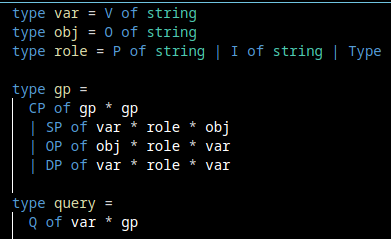
\includegraphics[scale=0.7]{pictures/queryType.png}
    \caption{tipo Query corrispondente alla sintassi delle query SPARQL CQ}
    \label{fig:querType}
\end{figure}


Per esempio, scrivendo questa query sul file di input:

\[ query \ x \ <- \ (x \ type \ Pizza \ AND \ x \ hasTopping \ y \ AND \ y \ type \ GorgonzolaTopping) \]

otteniamo il seguente tipo Query così costruito: 

\[ Q \  (V \ x, \\
    CP(SP(V \ x,\ TYPE, \ ,\ CP)\]

Introduciamo il tipo ClassExpression, definito ispirandosi alle regole di derivazione degli assiomi di Leiberger.
\begin{figure}[H]
    \centering
    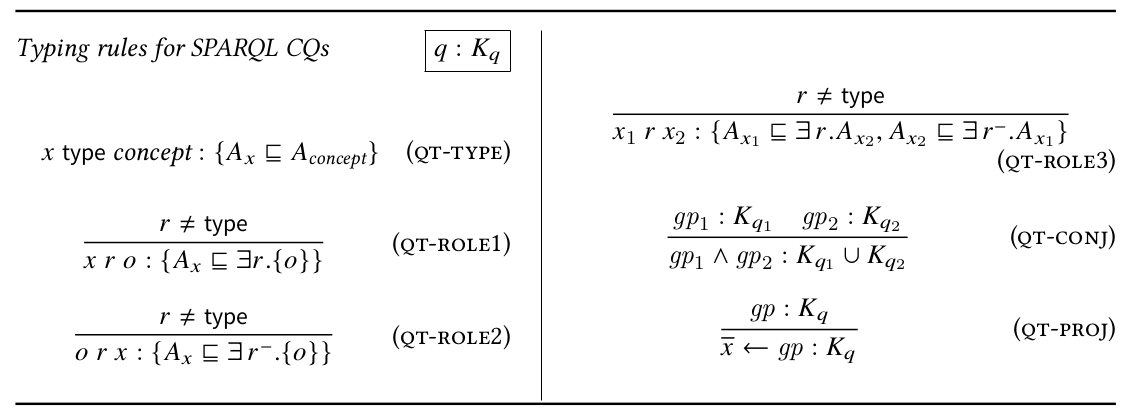
\includegraphics[width=\textwidth]{pictures/leinbergAxiom.png}
    \caption{Regole di derivazione degli assiomi di Leiberger}
    \label{fig:leinbergerAxiom}
\end{figure}

\begin{figure}[H]
    \centering
    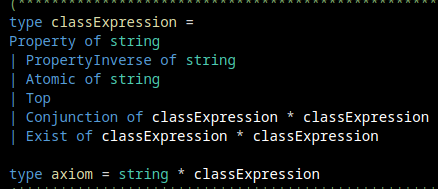
\includegraphics[width=\textwidth]{pictures/classExpressionType.png}
    \caption{Il tipo ClassExpression e Axiom}
    \label{fig:enter-label}
\end{figure}
Successivamente, il tipo Query viene convertito in una lista di Axiom dalla funzione axiomiserQuery, che implementa le regole di derivazione di Leinberger [\ref{fig:leinbergerAxiom}]\\ \\L'esempio diventa dunque:
\[ (x, Pizza) :: (x, Exist(Property(hasTopping),Atomic(y))) :: \]\[ (y, Exists(PropertyInverse(hasTopping), Atomic(x))) ::
      (y, GorgonzolaTopping) :: []
 \]
        
Infine, la lista di assiomi viene convertita in stringa secondo la sintassi \(A_{x} : C\), ove C è la traduzione in sintassi di Manchestern della classExpression corrispondente. 
\\\\ L'esempio diventa dunque
\[ x : Pizza : x : hasTopping \ SOME \ y : y : INVERSE \ hasTopping x : y : GorgonzolaTopping\]
Viene dunque invocato il modulo Reasoner e gli viene passato come parametro la lista in formato stringa. La risposta, true o false, viene poi mostrata a video all'utente. 

\newpage   
\section{Reasoner}
Il modulo Reasoner utilizza due risorse:
\begin{enumerate}
    \item Il file HermiT.jar\cite{HermiT}, che implementa il reasoner sviluppato dall'università di Oxford, capace di eseguire ragionamenti sulle ontologie.
    \item Il file DLQueryExample\cite{DLQueryExample} utilizzato per parsare una stringa in una ClassExpression, che è utilizzabile HermiT.
\end{enumerate}

Ma come funziona il modulo? Esso prende in input, in formato stringa, una lista di assiomi di Leinberger, ognuno forma \(A_{x} : C\), con semantica \( A_{x}\sqsubseteq C \).
\\\(A_{x}\) è un concetto atomico. "C" è una concept expression scritta nella "Manchester OWL syntax" \cite{ManchesterOWLSyntax}, e viene trasformato dal DLQueryParser in un oggetto ClassExpression. L'idea iniziale era di creare noi un parser che trasformasse una stringa in un oggetto ClassExpression, poi ci siamo imbattuti nella Manchester OWL syntax che presentava già un parsificatore capace di realizzare esattamente quello che volevamo. Allora ho adattato il tutto affinché lavorasse su questa particolare sintassi.

Utilizzando poi la OWLDataFactory (factory delle OWLApi che permette la costruzione di OWLAxiom e di dichiarare OWLClass) e HermiT\cite{HermiT}, dichiariamo all'interno dell'ontologia tutti i concetti atomici che compaiono negli assiomi di Leinberger\ref{fig:leinbergerSyntax}, corrispondenti alle variabili della query.

\begin{figure}[H]
    \centering
    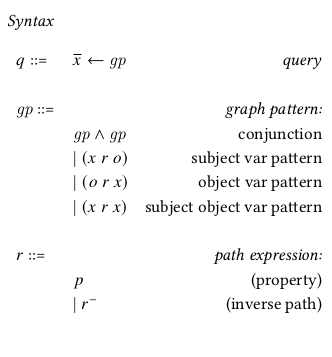
\includegraphics[scale=0.6]{pictures/leinbergSyntax}
    \caption{sintassi delle query \\ SPARQL CQ}
    \label{fig:leinbergerSyntax}
\end{figure}

Successivamente per ogni assioma creiamo un OWLSubClassOfAxiom, in cui viene specificata la relazione di sottoclasse tra il concetto atomico(le variabili) e la sua ClassExpression corrispondente(concept expression).

Infine chiediamo al reasoner HermiT di testare la soddisfacibilità di ogni concetto atomico presente negli assiomi di Leinberger. Se sono tutti soddisfacibili, allora significa che la query è abitabile, altrimenti non lo è.
    
    \newpage
    \section{Il linguaggio $\boldsymbol{\lambda_{DL}}$}
    Quando si effettua una computazione basata su ontologie, il processo di ragionamento è portato avanti a run time, e se si scoprono assiomi non soddisfacibili 
    il programma potrebbe essere soggetto a errori. Non è quindi possibile garantire che un'esecuzione termini correttamente, ovvero si otterrà il risultato aspettato. 
    Il nostro obiettivo è quello riuscire a catturare questi errori prima dell'esecuzione, andando ad assicurare una computazione senza errori run-time che dipendono dalla base di conoscenza. 
    Vorremmo quindi valutare vantaggi e efficienza di un controllo statico, sfruttando i sistemi di tipi per assicurare la correttezza statica del programma, rispetto a 
    un'ontologia basata sulle logiche descrittive (in particolare OWL). Sforzi verso questa direzioni sono stati già proposti nella tesi di dottorato di Martin Leinberger, 
    in cui propone un lambda calcolo tipato esteso con interrogazioni SPARQL a basi di triple RDF e costrutti della logica descrittiva come tipi chiamato $\lambda_{DL}$.
    \\ Il linguaggio garantisce di eseguire delle QUERY SPARQL che rispettano A-Box e T-Box dell'ontologia, spostando il controllo dell'abitabilità durante il type checking e
    permettendo di tipare i nodi ritornati dalle Query tramite le concept expressions della logica descrittiva.
    L'esempio successivo, preso dalla tesi di Leinberger, mostra un programma scritto in $\lambda_{DL}$ che espone chiaramente le potenzialità del linguaggio.
    \begin{figure}[h]
        \captionsetup{singlelinecheck = false}
        $K_4 = $\{Students $\sqsubseteq$ Person
        \\Professor $\sqsubseteq$ Person\}
        \begin{minted}[escapeinside=||,mathescape=true, autogobble]{ocaml}
            (head (query x |$\leftarrow$| x type Student)).x
        \end{minted}
        \caption{Programma in $\lambda_{DL}$ avente come knowledge base $K_4$}
    \end{figure}
    \\Il programma esegue una query SPARQL che ritorna una lista di mapping tra la variabile \textbf{x} e nodi del grafo RDF che rispettino il vincolo
    \textbf{x type Students}. Successivamente prendiamo il primo elemento della lista (\textbf{head}) e lo proiettiamo sulla variabile \textbf{x} (\textbf{(...).x}).
    Il sistema di tipo ci permette di:
    \begin{itemize}
        \item stabilire la correttezza della query, costruendo degli assiomi dalla sua struttura e richiamando un reasoner.
        \item dare un tipo ai nodi ritornati dalla query. Nel nostro esempio tutta l'espressione è di tipo \textbf{Students} e grazie al subtyping e al fatto
            che nella knowledge base sappiamo che Students $\sqsubseteq$ Person è anche ti tipo \textbf{Person}.
    \end{itemize}
    L'implementazione si concentra solo sul type system, i riferimenti agli aspetti più teorici del linguaggio insieme alla sintassi e le regole di valutazione
    si possono trovare nella tesi di Leiberger.
    Vale la pena per\`o accennare che il linguaggio è corretto, ovvero un termine chiuso e ben tipato non si blocca durante la valutazione.
    La corretteza è dimostrata da Leinberger attraverso due teoremi:
    \begin{theorem}
        (Progress in $\lambda_{DL}$): sia t un termine ben tipato e chiuso. se t non è un valore, allora esiste una termine t' tale che
        t $\xrightarrow[]{\text{K}}$ t'. Se $\Gamma$, K $\vdash$ t : T, allora t è un valore o un termine contenente head nil[T] e tail nil[T] oppure esiste
        un t' per cui t $\xrightarrow[]{\text{K}}$ t'
    \end{theorem}
    \begin{theorem}
        (Preservation in $\lambda_{DL}$): Sia t un termine e T un tipo. Se un tipo è assegnato a t, scritto $\Gamma,K \vdash t : T$ e t $\xrightarrow[]{\text{K}}$ t'
        allora, $\Gamma,K \vdash t' : T$
    \end{theorem}
    Entrambe le dimostrazioni sono per induzione su $\Gamma,K \vdash t : T$ e i dettagli si possono trovare nella tesi di Leinberger.
\newpage
\section{Type Checking} \label{sec:Type Checking}
        Per implementare il type checking abbiamo usato come base il lambda calcolo tipato proposto dal libro di \textbf{Benjamin C. Pierce "Types and Programming Languages"}.
        Nella tesi parleremo strettamente delle regole di tipo e della loro implementazione per quanto riguarda la valutazioni si veda il libro di Pierce e la tesi di Leinberger.
        Il linguaggio presenta le principali caratteristiche di un \textbf{ $\boldsymbol{\lambda}$-calcolo tipato} con l'aggiunta dei \textbf{Record}, le \textbf{Liste} e le \textbf{Query SPARQL}.
        \begin{figure}[h] 
            \begin{minted}{ocaml}
                type Term =
                      TmVar of info * int * int 
                    | TmTrue of info 
                    | TmFalse of info 
                    | TmIf of info * term * term * term 
                    | TmRecord of info * (string * term) list 
                    | TmProj of info * term * string 
                    | TmAbs of info * string * ty * term 
                    | TmApp of info * term * term 
                    | TmLet of info * string * term * term 
                    | TmFix of info * term 
                    | TmZero of info 
                    | TmSucc of info * term 
                    | TmPred of info * term 
                    | TmIsZero of info * term 
                    | TmNil of info * ty 
                    | TmCons of info * term * term 
                    | TmIsNil of info * term 
                    | TmHead of info * term 
                    | TmTail of info * term  
                    | TmQuery of info * var * gp
                    | TmRoleProj of info * term * role
                    | TmEq of info * term * term
                    | TmNode of info * string
            \end{minted}
        \caption{termini del $\lambda_{DL}$}
        \end{figure}
        TmRecord e quello che ci permette di avere nel nostro linguaggio termini come:
        \begin{minted}{OCaml}
        {x = 4; y = 0; z = 4}
        \end{minted}
        dove $x, y, z$ sono le etichette del record, mentre $4, 0, 4$ sono i termini associati alle etichette. Nella implementazione corrispondono rispettivamente alla
        stringa e al termine della lista. TmProj invece è la proiezione di un record su una etichetta, quindi riprentendo dall'esmpio precedente 
        \begin{minted}{Ocaml}
        {x = 4; y = 0; z = 4}.x
        \end{minted}
        il record proiettato su x, come ci si aspetta, sarà valutato nel valore associato alla etichetta: 4.
        Le liste sono costruite ricorsivamente con \textbf{TmNil} e \textbf{TmCons} e sono presenti delle operazioni sulle liste espresse dai termini \textbf{TmIsNil},
        \textbf{TmHead} e \textbf{TmTail}
        \begin{figure}[h]
            \begin{minted}[escapeinside =|, autogobble]{python}
                [1, 0]        TmCons (TmSucc (TmZero)) (TmCons (TmZero) (TmNil))
                head  [1, 0]  TmHead (TmCons (TmSucc (TmZero)) (TmCons (TmZero) (TmNil)))
                tail  [1, 0]  TmTail (TmCons (TmSucc (TmZero)) (TmCons (TmZero) (TmNil)))
                isNil [1, 0]  TmIsNil (TmCons (TmSucc (TmZero)) (TmCons (TmZero) (TmNil)))
            \end{minted}
        \caption{esempi di termini con liste}
        \end{figure}
        Infine le query sono implementate come descritto nella sezione precedente.
        \\I tipi hanno un datatype apposito. Oltre ad avere i classici tipi booleani (TyBool), numeri natoruali (TyNat) e il tipo freccia (TyArr) 
        sono presenti i tipi per i nuovi costrutti (TyRecord, TyList, TyConcept). Il tipo \textbf{Top} è usato per il subtyping, in particolare per
        qualsiasi tipo $T$ vale che $\boldsymbol{T <: Top}$. La figura sottostante mostra il datatype costruito in OCaml.
        \begin{minted}{ocaml}
            type Ty =
                  TyTop 
                | TyBool 
                | TyRecord of (string * ty) list 
                | TyArr of ty * ty 
                | TyNat 
                | TyList of ty
                | TyConcept of ce
        \end{minted}
        Alcuni esempi di tipi assegnati ai relativi termini possono essere:
        \begin{minted}{ocaml}
            {x = 4; y = 0; z = 4} : {x : Nat, y : Nat, z = Nat}
            [1, 0] : List Nat
            query x <- x type students : List {x : Ax}
        \end{minted}
        dove i tipi segnati sono un versione semplificata e più leggibile per indicare il termine costruito dal datatype ty:
        \begin{minted}{ocaml}
            TyRecord([("x", TyNat); ("y", TyNat); ("z", TyNat)])
            TyList TyNat
            TyConcept Atomic("x")
        \end{minted}
        Ora che abbiamo introdotto i costruttori di tipi utilizzati possiamo paralre dell'algoritmo di typing.
        Come suggerito dal libro "Types and Programming Languages" viene utilizzata una funzione ricorsiva per determinare il tipo di un termine da un contesto
        inizialmente vuoto.
        \begin{minted}{ocaml}
            typeof : Context -> Term -> Ty
        \end{minted}
        typeof effettua pattern matching sul termine passato come argomento per decidere quale regola applicare. La maggior parte delle regole sono puramente
        sintattiche quindi typeof è sufficiente per la loro implementazione, altre come le regole di subtyping o [T-ADD] è necessario utilizzare funzioni di supporto
        oppure modificare l'implementazione delle regole precedenti. Un semplice esempio di implementazione di una regola di tipo è quello di [T-APP].
        $$\myruleN{\Gamma \vdash t_1 : T_1 \rightarrow T_2 \quad \Gamma \vdash t_2 : T_1}{\Gamma \vdash t_1 \: t_2 : T_2}{T-APP}$$
        la cui implementazione diventerà:
        \begin{minted}[escapeinside=||,mathescape=true, autogobble]{ocaml}
            let rec typeof ctx t =
                match t with
                |$\vdots $|
                TmApp(fi,t1,t2) ->
                    let tyT1 = typeof ctx t1 in
                    let tyT2 = typeof ctx t2 in
                    (match ctx tyT1 with
                        TyArr(tyT11,tyT12) ->
                          if subtype ctx tyT2 tyT11 then tyT12
                          else error fi "parameter type mismatch"
                        | _ -> error fi "arrow type expected")

                |$\vdots$|
        \end{minted}
        Prima attraverso pattern matching si controlla che il termine passato sia un'applicazione tra altri due termini $t1$ e $t2$. Successivamente
        viene effettuata la chiamata ricorsiva su $t1$ e $t2$ per ottenere i loro tipi $tyT1$ e $tyT2$ rispettivamente. Effettuando di nuovo pattern matching
        su $tyT1$ si verifica che sia un tipo freccia $tyT11 \rightarrow tyT12$. Infine se $tyT2 <: tyT11$ allora si può stabilire che $t1 \; t2$ ha tipo $tyT12$.
        Come si vede dalla implementazione di [T-APP] è stata utilizzata una funzione per verificare il subtyping, ritornando true se e solo se $Ty_1 <: Ty_2$. 
        \begin{minted}{ocaml}
            subtype : Context -> Ty -> Ty -> Bool
        \end{minted}
        Il linguaggio $\lambda_{DL}$ presenta il subtyping classico tra funzioni, record e liste le cui regole si possono trovare sia nella tesi di Leinberger che
        in "Types and Programming Languages". L'implementazione della funzione \textbf{subtype} è molto diretta rispetto alle regole. Come per \textbf{typeof}
        si procede con il pattern matching tra i tipi passati come argomento e confrontando la loro struttura si può stabilire se sono in relazione di sottotipo.
        Per esempio la regola \textbf{[S-LIST]}
        $$\myruleN{T <: T'}{List \; T <: List \; T'}{S-LIST}$$
        \\ viene implementata con con:
        \begin{minted}[escapeinside =**, mathescape=true, autogobble]{ocaml}
            let rec subtype ctx tyS tyT =
                tyeqv ctx tyS tyT ||
                match (tyS,tyT) with
                    *$\vdots$*
                     (TyList(tyS1),TyList(tyT1)) -> subtype ctx tyS1 tyT1
                    *$\vdots$*
        \end{minted}
        La funzione tyeqv controlla l'ugualianza tra due tipi siccome la relazione di subtyping è riflessiva. l'ultime due funzioni di supporto
        utilizzate per il typing calcolano il least upper bound (\textbf{join}) e il greatest lower bound (\textbf{meet}) tra due tipi.
        \begin{minted}{ocaml}
            meet : Context -> Ty -> Ty -> Ty
            join : Context -> Ty -> Ty -> Ty
        \end{minted}
        La figura sottostante mostra le regole di tipo aggiunte da Leinberger nel $\lambda_{DL}$ e nelle sottosezioni successive analizzeremo regola per regola
        il loro significato e ne mostreremo una possibile implementazione.  
        \textbf{aggiungere correttezza, obiettivo del type system e nelle introduzioni introdurre con esempi il linguaggio, aggiungere i riferimenti alla sezione precedente}
        \begin{figure}[h]
        \[\begin{array}{c}
            \myruleN{\Gamma,K \vdash t_1 : C_1 \quad K \vDash C_1 \sqsubseteq \exists r . \top}
            {\Gamma,K \vdash t_1.r : \textrm{List}(\exists r^- . C_1)}
            {T-PROJ}
            \qquad
            \myruleN{\Gamma,K \vdash : C \quad \Gamma,K \vdash t_2 : D}
            {\Gamma, K \vdash t_1 = t_2 : \textrm{Bool}}
            {T-EQ-NOM}
            \qquad
            \\\\
            \myruleN{\Gamma,K \vdash t_1 : \Pi_1 \quad \Gamma,K \vdash t_2 : \Pi_1}
            {\Gamma,K \vdash t_1 = t_2 : \textrm{Bool}}
            {T-EQ-PRIM}
            \qquad
            \myruleN{}{\Gamma,K \vdash o : \{o\}}{T-NOMINAL}
            \\\\
            \myruleN{q:K_q \quad \textrm{head}(q) = \{l_i^{i \in 1...m}\} \quad \forall x \in \textrm{Vars}(q) : K \cup K_q \nvDash A_x \sqsubseteq \bot}
            {\Gamma,K \cup K_q \vdash \textrm{query} \; q : \{l_i : A_{l_i}^{i \in 1...m}\} list}
            {T-QUERY}
            \\\\
            \myruleN{\Gamma,K \cup \{A_i \sqsubseteq C_i^{i \in 1...n}\} \vdash t : A_j^{1 \leq j \leq n} \quad K \cup \{A_i \sqsubseteq C_i^{i \in 1...n}\} \vDash A_j \sqsubseteq D^{1 \leq j \leq n}}
            {\Gamma,K \vdash t : D}
            {T-ADD}
            \\\\
            \myruleN{K \vDash C \sqsubseteq D}{K \vdash C <: D}{S-CONCEPT}
        \end{array}\]
        \caption{nuove regole di tipo per $\lambda_{DL}$}
        \end{figure}
        \subsection{La regola [T-PROJ]}
            L'implementazione della regola [T-PROJ] segue alla lettera la definizione teorica in particolare abbiamo che la condizione $\Gamma,K \vdash t_1 : C_1$
            è verificata attraverso il pattern matching (.1) in cui controlliamo che il tipo $t$ sia una concept expression \textbf{TyConcept(C)}. La seconda ipotesi
            $K \vDash C_1 \sqsubseteq \exists r . \top$ invece richiede la creazione di una nuova funzione:
            \begin{minted}[escapeinside=||,mathescape=true, framesep=4mm, autogobble]{ocaml}
                subconcept : ConceptExpression -> ConceptExpression -> Bool
            \end{minted}
            la funzione subconcept prende in input due concept expression $C_1$ e $C_2$ e ritorna $true$ se e solo se $C_1 \sqsubseteq C_2$. Quindi passando a subconcept
            \textbf{C} e \textbf{Exist(Property(s), Top)} (.2) come argomento verifichiamo la seconda condizione.
            \\Infine le conclusioni della regola $\Gamma,K \vdash t_1.r : \textrm{List}(\exists r^- . C_1)$ affermano facendo la proiezione del termine $T_1$ attraverso $r$
            otteniamo una lista di concept expression $\exists r^- . C_1$, per questo motivo la funzione typeof ritorna  \textbf{TyList(TyConcept(Exist(PropertyInverse(s), c)))} (.3).
            \begin{figure}[h] 
                \begin{minted}[escapeinside=||,mathescape=true, frame=lines, framesep=4mm, autogobble]{ocaml}
                    let rec typeof ctx t =
                        match t with
                        |$\vdots $|
                        TmRoleProj(fi, t, Property(s)) ->
                            (match typeof ctx t with
                            TyConcept(C) as t ->                                        .1
                                if subconcept C Exist(Property(s), Top) then            .2
                                    TyList(TyConcept(Exist(PropertyInverse(s), c)))     .3
                                else error fi "argument of role projection 
                                                is not a proper subconcept")
                            _ -> error fi "argument of role projection 
                                            is not a Concept Expression"
                        |$\vdots$|
                \end{minted}
            \caption{implementazione OCaml della regola [T-PROJ]}
            \end{figure}

            \subsection{La regola [T-QUERY]}
            [T-QUERY] è la regola utilizzata per derivare il tipo di una query SPARQL. Per semplicità, rispetto alla teoria, prendiamo in considerazione solo le query
            aventi una variabile, ovvero dove l'insieme $Head(q)$ contiene un solo elemento. Anche questa regola richiede di consultare un reasoner per stabilire se
            gli assiomi generati dal typing della query q siano soddisfacibili $\forall x \in \textrm{Vars}(q) : K \cup K_q \nvDash A_x \sqsubseteq \bot$.
            Nella definizione la funzione $Vars(q)$ ritorna l'insieme di tutte le variabili utilizzate nella query.
            \begin{figure}[h]
                \begin{minted}[escapeinside=||,mathescape=true, frame=lines, framesep=4mm, autogobble]{ocaml}
                    let rec typeof ctx t =
                        match t with
                        |$\vdots $|
                        TmQuery(fi, var, gp) ->
                            if allSatisfiable(axioms(gp), var) then
                            TyList(TyRecord(var, TyConcept(Atomic var))) else
                                error fi "axioms unsatisibale"
                        |$\vdots$|
                \end{minted}
            \caption{implementazione OCaml della regola [T-QUERY]}
            \end{figure}
            \\Nella implementazione, per verificare le ipotesi utilizziamo due funzioni di supporto. la prima:
            \begin{minted}{OCaml}
            axioms: Gp -> Axiom List
            \end{minted}
            ritorna la lista degli assiomi dal graph pattern della query. mentre la seconda
            \begin{minted}{OCaml}
            allSatisfiable: Axioms List -> Var -> Bool
            \end{minted}
            è la funzione che interroga la knowledge base per verificare che la lista degli assiomi sia soddisfacibile. Infine una volta verificate le ipotesi possiamo
            ritornare
            \\\textbf{TyList(TyRecord(var, TyConcept(Atomic \; var)))} che corrisponde a $\Gamma,K \cup K_q \vdash \textrm{query} \; q : \{l_i : A_{l_i}^{i \in 1...m}\} list$
            con l'unica differenza che nella nostra implementazione i record contengono una sola label, quella della unica variabile in $Head(q)$. Abbiamo deciso di
            mantenere la lista di record nonostante la nostra semplificazine sulle query per rendere un futuro aggiornamento facile da implementare.
            \subsection{La regola [T-ADD]}
            [T-ADD] è la regola la cui implementazione è più interessante. Siccome non siamo di fronte ad una regola puramente sintattica
            non è possibile fare pattern matching sul termine per capire quando applicarla.
            Prima di parlare dell'implementazione è importante capire a cosa serve e come viene utilizzada: [T-QUERY] assegna alle variabili in testa alla query
            il tipo concept expression $A_x$ quando abbiamo un assioma nella query della forma $K_q = A_x \sqsubseteq D$, ma $A_x$ non sono propriamente da usare sintatticamente nel programma.
            \\L'obiettivo è dare un significato al tipo $A_x$, in modo simile a una classica regola di subtyping. Quindi è possibile assegnate una concept espression $D$
            a un termine t solo se è possibile assegnare a t $A_x$ usando una knowledge base $\Gamma,K \cup \{A_i \sqsubseteq C_i^{i \in 1...n}\} \vdash t : A_j^{1 \leq j \leq n}$
            e se K $\cup \{A_i \sqsubseteq C_i^{i \in 1...n}\} \vDash A_j \sqsubseteq D^{1 \leq j \leq n}$.
            \\Come suggerito da Leinberger, abbiamo implementato la regola aggiungendo gli assiomi $K_q$ alla knowledge base durante la funzione \textbf{allSatisfiable}.
            così insieme alla regola \textbf{S-CONCEPT} è possibile risalire alla concept $D$ senza avere bisogno di [T-ADD].
            \subsection{La regola [S-CONCEPT]}
            Il linguaggio cotruito da Leinberger permette il subtyping tipi, quindi oltre a quello tra tipi classici è stato necessario aggiungere un modo per gestire
            anche quello tra le concept expression.
            \begin{figure}[h]
                \begin{minted}[escapeinside=||,mathescape=true, frame=lines, framesep=4mm, autogobble]{ocaml}
                    let rec subtype ctx tyS tyT =
                        tyeqv ctx tyS tyT ||
                        match (tyS,tyT) with
                        |$\vdots $|
                            (TyConcept(ceS1),TyConcept(ceT1)) -> subconcept ceS1 ceT1
                        |$\vdots$|
                \end{minted}
            \caption{implementazione OCaml della regola [S-CONCEPT]}
            \end{figure}
            Nella implementazione richiamiamo la funzione subconcept per il controllo della ipotesi $K \vDash C \sqsubseteq D$. La differenza maggiore rispetto alla teoria
            risiede nel fatto che anche in questo caso [S-CONCEPT] non è una regola sintattica. La funzione subtype ha tipo:
            \begin{minted}[]{ocaml}
                subtype : Context -> Ty -> Ty -> Bool
            \end{minted}
            Prende in input un contesto e due tipi e ritorna $true$ se e solo se $K \vDash C \sqsubseteq D$. la funzione subtype viene poi richiamata su tutte le regole
            in cui il subtyping è utilizzabile. Ad esempio nella regola [T-APP] si controlla che l'argomento passato a una astrazione sia sottotipo del tipo atteso dalla astrazione (\textbf{Controvarianza}).
            \begin{minted}[escapeinside=||,mathescape=true, frame=lines, framesep=4mm, autogobble]{ocaml}
                let rec typeof ctx t =
                    match t with
                    |$\vdots $|
                    TmApp(fi,t1,t2) ->
                    let tyT1 = typeof ctx t1 in
                    let tyT2 = typeof ctx t2 in
                    (match ctx tyT1 with
                        TyArr(tyT11,tyT12) ->
                          if subtype ctx tyT2 tyT11 then tyT12
                          else error fi "parameter type mismatch"
                        _ -> error fi "arrow type expected")
                    |$\vdots$|
            \end{minted}












        
        
\clearemptydoublepage

\chapter[Chapter name for Index]{Lorem Ipsum}
Lorem ipsum dolor sit amet\footnote{first foot note}, consectetur adipiscing elit. Sed dui sem, aliquam id ultricies sit amet, fermentum at magna. Aenean vitae rhoncus leo. Fusce gravida consequat lacus, a porta risus bibendum semper. Morbi eget auctor velit. Pellentesque eu lacinia nisi. Maecenas sed orci eu erat porta imperdiet ac non dui. Pellentesque a odio ac quam euismod tempor. Nulla in dapibus mauris, a sodales ex. In imperdiet enim sed ornare sollicitudin. Pellentesque\footnote{another foot note} habitant morbi tristique senectus et netus et malesuada fames ac turpis egestas. Donec vehicula metus eu nisi ornare euismod. Proin at ex non ex iaculis porta.

\section[Section name]{Section name for index}
Lorem ipsum dolor sit amet, consectetur adipiscing elit. Sed dui sem, aliquam id ultricies sit amet, fermentum at magna. Aenean vitae rhoncus leo. Fusce gravida consequat lacus, a porta risus bibendum semper. Morbi eget auctor velit. Pellentesque eu lacinia nisi. Maecenas sed orci eu erat porta imperdiet ac non dui. Pellentesque a odio ac quam euismod tempor. Nulla in dapibus mauris, a sodales ex. In imperdiet enim sed ornare sollicitudin. Pellentesque habitant morbi tristique senectus et netus et malesuada fames ac turpis egestas. Donec vehicula metus eu nisi ornare euismod. Proin at ex non ex iaculis porta.

Here I want to test\cite{einstein} some\cite{latexcompanion} quote\cite{knuthwebsite}

\subsection[Subsection name]{Subsection name for index}
Nulla interdum molestie bibendum. Quisque condimentum justo quis lectus pretium, eget porttitor odio elementum. In dignissim sed justo et congue. In pulvinar feugiat odio eu vehicula. In ut malesuada est, sit amet porttitor dolor. Donec ullamcorper libero eros, vitae blandit nibh pellentesque quis. Aliquam aliquet ex id sapien lobortis, at molestie sem commodo. Donec quis accumsan lectus. Sed eget turpis id mi iaculis accumsan. Maecenas eget rutrum leo. Nam eu purus vitae lorem semper vestibulum. Phasellus mattis euismod faucibus. Vestibulum ornare sem a mattis placerat. Donec interdum blandit erat, eu iaculis risus cursus sed. Donec magna sem, finibus nec scelerisque nec, auctor in turpis.

\subsubsection[Subsubsection name]{Subsubsection name for index}
In lobortis augue porta dui venenatis sollicitudin. In sagittis quis ipsum non dictum. Sed tempus, quam non vehicula dictum, mauris nisl posuere metus, eu lobortis odio risus at dui. Nullam non ante vulputate nulla ultrices euismod eu a diam. Cum sociis natoque penatibus et magnis dis parturient montes, nascetur ridiculus mus. Nulla nec augue a risus viverra mattis. Ut tincidunt egestas nulla at semper. Fusce pretium, leo quis consectetur viverra, arcu lectus ornare leo, quis commodo ex risus sit amet velit. Nullam finibus lorem in mi tincidunt, sed feugiat lectus tincidunt. In hac habitasse platea dictumst. Sed quis auctor odio, at sodales nunc. Donec vulputate massa sit amet dolor sollicitudin, vel pretium quam scelerisque. Nullam et massa eleifend, venenatis ante vitae, ornare libero. Suspendisse potenti. Nam ante lacus, porttitor vel turpis quis, pellentesque auctor velit.

Morbi eget elementum tellus. Sed varius lacus ac nulla maximus, et varius lacus varius. Nulla faucibus magna sit amet magna auctor, vitae placerat turpis imperdiet. Duis blandit bibendum tellus nec accumsan. Aliquam arcu nulla, efficitur vitae sodales eu, tincidunt ac tortor. Cras gravida vulputate porttitor. Etiam ornare est at efficitur convallis. Quisque pulvinar tellus pulvinar lacus tristique, bibendum dapibus velit ultricies. Suspendisse id faucibus dui. Sed quis convallis dui. Etiam aliquam suscipit eros id pellentesque. Aliquam a suscipit leo, sit amet convallis dui. Donec sed pretium quam. Mauris nec tincidunt mi, in feugiat quam.

Sed convallis pulvinar dui et ullamcorper. Maecenas facilisis, ante a tristique convallis, nunc ipsum fermentum odio, a auctor ligula risus ut nibh. Praesent sit amet tempus metus. Proin enim ipsum, mollis in nunc sed, tempus tempor magna. Nam ultricies lacus et porttitor bibendum. Suspendisse sit amet placerat nibh. Curabitur rutrum massa eu tortor sodales iaculis. Mauris sit amet odio eget velit tempus auctor. Pellentesque nec posuere neque. Nam in orci vehicula, ullamcorper sapien quis, pellentesque mauris. Sed eu porta ex. 

In lobortis augue porta dui venenatis sollicitudin. In sagittis quis ipsum non dictum. Sed tempus, quam non vehicula dictum, mauris nisl posuere metus, eu lobortis odio risus at dui. Nullam non ante vulputate nulla ultrices euismod eu a diam. Cum sociis natoque penatibus et magnis dis parturient montes, nascetur ridiculus mus. Nulla nec augue a risus viverra mattis. Ut tincidunt egestas nulla at semper. Fusce pretium, leo quis consectetur viverra, arcu lectus ornare leo, quis commodo ex risus sit amet velit. Nullam finibus lorem in mi tincidunt, sed feugiat lectus tincidunt. In hac habitasse platea dictumst. Sed quis auctor odio, at sodales nunc. Donec vulputate massa sit amet dolor sollicitudin, vel pretium quam scelerisque. Nullam et massa eleifend, venenatis ante vitae, ornare libero. Suspendisse potenti. Nam ante lacus, porttitor vel turpis quis, pellentesque auctor velit.

Morbi eget elementum tellus. Sed varius lacus ac nulla maximus, et varius lacus varius. Nulla faucibus magna sit amet magna auctor, vitae placerat turpis imperdiet. Duis blandit bibendum tellus nec accumsan. Aliquam arcu nulla, efficitur vitae sodales eu, tincidunt ac tortor. Cras gravida vulputate porttitor. Etiam ornare est at efficitur convallis. Quisque pulvinar tellus pulvinar lacus tristique, bibendum dapibus velit ultricies. Suspendisse id faucibus dui. Sed quis convallis dui. Etiam aliquam suscipit eros id pellentesque. Aliquam a suscipit leo, sit amet convallis dui. Donec sed pretium quam. Mauris nec tincidunt mi, in feugiat quam.

Sed convallis pulvinar dui et ullamcorper. Maecenas facilisis, ante a tristique convallis, nunc ipsum fermentum odio, a auctor ligula risus ut nibh. Praesent sit amet tempus metus. Proin enim ipsum, mollis in nunc sed, tempus tempor magna. Nam ultricies lacus et porttitor bibendum. Suspendisse sit amet placerat nibh. Curabitur rutrum massa eu tortor sodales iaculis. Mauris sit amet odio eget velit tempus auctor. Pellentesque nec posuere neque. Nam in orci vehicula, ullamcorper sapien quis, pellentesque mauris. Sed eu porta ex. 
In lobortis augue porta dui venenatis sollicitudin. In sagittis quis ipsum non dictum. Sed tempus, quam non vehicula dictum, mauris nisl posuere metus, eu lobortis odio risus at dui. Nullam non ante vulputate nulla ultrices euismod eu a diam. Cum sociis natoque penatibus et magnis dis parturient montes, nascetur ridiculus mus. Nulla nec augue a risus viverra mattis. Ut tincidunt egestas nulla at semper. Fusce pretium, leo quis consectetur viverra, arcu lectus ornare leo, quis commodo ex risus sit amet velit. Nullam finibus lorem in mi tincidunt, sed feugiat lectus tincidunt. In hac habitasse platea dictumst. Sed quis auctor odio, at sodales nunc. Donec vulputate massa sit amet dolor sollicitudin, vel pretium quam scelerisque. Nullam et massa eleifend, venenatis ante vitae, ornare libero. Suspendisse potenti. Nam ante lacus, porttitor vel turpis quis, pellentesque auctor velit.

Morbi eget elementum tellus. Sed varius lacus ac nulla maximus, et varius lacus varius. Nulla faucibus magna sit amet magna auctor, vitae placerat turpis imperdiet. Duis blandit bibendum tellus nec accumsan. Aliquam arcu nulla, efficitur vitae sodales eu, tincidunt ac tortor. Cras gravida vulputate porttitor. Etiam ornare est at efficitur convallis. Quisque pulvinar tellus pulvinar lacus tristique, bibendum dapibus velit ultricies. Suspendisse id faucibus dui. Sed quis convallis dui. Etiam aliquam suscipit eros id pellentesque. Aliquam a suscipit leo, sit amet convallis dui. Donec sed pretium quam. Mauris nec tincidunt mi, in feugiat quam.

Sed convallis pulvinar dui et ullamcorper. Maecenas facilisis, ante a tristique convallis, nunc ipsum fermentum odio, a auctor ligula risus ut nibh. Praesent sit amet tempus metus. Proin enim ipsum, mollis in nunc sed, tempus tempor magna. Nam ultricies lacus et porttitor bibendum. Suspendisse sit amet placerat nibh. Curabitur rutrum massa eu tortor sodales iaculis. Mauris sit amet odio eget velit tempus auctor. Pellentesque nec posuere neque. Nam in orci vehicula, ullamcorper sapien quis, pellentesque mauris. Sed eu porta ex. 
In lobortis augue porta dui venenatis sollicitudin. In sagittis quis ipsum non dictum. Sed tempus, quam non vehicula dictum, mauris nisl posuere metus, eu lobortis odio risus at dui. Nullam non ante vulputate nulla ultrices euismod eu a diam. Cum sociis natoque penatibus et magnis dis parturient montes, nascetur ridiculus mus. Nulla nec augue a risus viverra mattis. Ut tincidunt egestas nulla at semper. Fusce pretium, leo quis consectetur viverra, arcu lectus ornare leo, quis commodo ex risus sit amet velit. Nullam finibus lorem in mi tincidunt, sed feugiat lectus tincidunt. In hac habitasse platea dictumst. Sed quis auctor odio, at sodales nunc. Donec vulputate massa sit amet dolor sollicitudin, vel pretium quam scelerisque. Nullam et massa eleifend, venenatis ante vitae, ornare libero. Suspendisse potenti. Nam ante lacus, porttitor vel turpis quis, pellentesque auctor velit.

Morbi eget elementum tellus. Sed varius lacus ac nulla maximus, et varius lacus varius. Nulla faucibus magna sit amet magna auctor, vitae placerat turpis imperdiet. Duis blandit bibendum tellus nec accumsan. Aliquam arcu nulla, efficitur vitae sodales eu, tincidunt ac tortor. Cras gravida vulputate porttitor. Etiam ornare est at efficitur convallis. Quisque pulvinar tellus pulvinar lacus tristique, bibendum dapibus velit ultricies. Suspendisse id faucibus dui. Sed quis convallis dui. Etiam aliquam suscipit eros id pellentesque. Aliquam a suscipit leo, sit amet convallis dui. Donec sed pretium quam. Mauris nec tincidunt mi, in feugiat quam.

Sed convallis pulvinar dui et ullamcorper. Maecenas facilisis, ante a tristique convallis, nunc ipsum fermentum odio, a auctor ligula risus ut nibh. Praesent sit amet tempus metus. Proin enim ipsum, mollis in nunc sed, tempus tempor magna. Nam ultricies lacus et porttitor bibendum. Suspendisse sit amet placerat nibh. Curabitur rutrum massa eu tortor sodales iaculis. Mauris sit amet odio eget velit tempus auctor. Pellentesque nec posuere neque. Nam in orci vehicula, ullamcorper sapien quis, pellentesque mauris. Sed eu porta ex. 
In lobortis augue porta dui venenatis sollicitudin. In sagittis quis ipsum non dictum. Sed tempus, quam non vehicula dictum, mauris nisl posuere metus, eu lobortis odio risus at dui. Nullam non ante vulputate nulla ultrices euismod eu a diam. Cum sociis natoque penatibus et magnis dis parturient montes, nascetur ridiculus mus. Nulla nec augue a risus viverra mattis. Ut tincidunt egestas nulla at semper. Fusce pretium, leo quis consectetur viverra, arcu lectus ornare leo, quis commodo ex risus sit amet velit. Nullam finibus lorem in mi tincidunt, sed feugiat lectus tincidunt. In hac habitasse platea dictumst. Sed quis auctor odio, at sodales nunc. Donec vulputate massa sit amet dolor sollicitudin, vel pretium quam scelerisque. Nullam et massa eleifend, venenatis ante vitae, ornare libero. Suspendisse potenti. Nam ante lacus, porttitor vel turpis quis, pellentesque auctor velit.

Morbi eget elementum tellus. Sed varius lacus ac nulla maximus, et varius lacus varius. Nulla faucibus magna sit amet magna auctor, vitae placerat turpis imperdiet. Duis blandit bibendum tellus nec accumsan. Aliquam arcu nulla, efficitur vitae sodales eu, tincidunt ac tortor. Cras gravida vulputate porttitor. Etiam ornare est at efficitur convallis. Quisque pulvinar tellus pulvinar lacus tristique, bibendum dapibus velit ultricies. Suspendisse id faucibus dui. Sed quis convallis dui. Etiam aliquam suscipit eros id pellentesque. Aliquam a suscipit leo, sit amet convallis dui. Donec sed pretium quam. Mauris nec tincidunt mi, in feugiat quam.

Sed convallis pulvinar dui et ullamcorper. Maecenas facilisis, ante a tristique convallis, nunc ipsum fermentum odio, a auctor ligula risus ut nibh. Praesent sit amet tempus metus. Proin enim ipsum, mollis in nunc sed, tempus tempor magna. Nam ultricies lacus et porttitor bibendum. Suspendisse sit amet placerat nibh. Curabitur rutrum massa eu tortor sodales iaculis. Mauris sit amet odio eget velit tempus auctor. Pellentesque nec posuere neque. Nam in orci vehicula, ullamcorper sapien quis, pellentesque mauris. Sed eu porta ex. 
In lobortis augue porta dui venenatis sollicitudin. In sagittis quis ipsum non dictum. Sed tempus, quam non vehicula dictum, mauris nisl posuere metus, eu lobortis odio risus at dui. Nullam non ante vulputate nulla ultrices euismod eu a diam. Cum sociis natoque penatibus et magnis dis parturient montes, nascetur ridiculus mus. Nulla nec augue a risus viverra mattis. Ut tincidunt egestas nulla at semper. Fusce pretium, leo quis consectetur viverra, arcu lectus ornare leo, quis commodo ex risus sit amet velit. Nullam finibus lorem in mi tincidunt, sed feugiat lectus tincidunt. In hac habitasse platea dictumst. Sed quis auctor odio, at sodales nunc. Donec vulputate massa sit amet dolor sollicitudin, vel pretium quam scelerisque. Nullam et massa eleifend, venenatis ante vitae, ornare libero. Suspendisse potenti. Nam ante lacus, porttitor vel turpis quis, pellentesque auctor velit.

Morbi eget elementum tellus. Sed varius lacus ac nulla maximus, et varius lacus varius. Nulla faucibus magna sit amet magna auctor, vitae placerat turpis imperdiet. Duis blandit bibendum tellus nec accumsan. Aliquam arcu nulla, efficitur vitae sodales eu, tincidunt ac tortor. Cras gravida vulputate porttitor. Etiam ornare est at efficitur convallis. Quisque pulvinar tellus pulvinar lacus tristique, bibendum dapibus velit ultricies. Suspendisse id faucibus dui. Sed quis convallis dui. Etiam aliquam suscipit eros id pellentesque. Aliquam a suscipit leo, sit amet convallis dui. Donec sed pretium quam. Mauris nec tincidunt mi, in feugiat quam.

Sed convallis pulvinar dui et ullamcorper. Maecenas facilisis, ante a tristique convallis, nunc ipsum fermentum odio, a auctor ligula risus ut nibh. Praesent sit amet tempus metus. Proin enim ipsum, mollis in nunc sed, tempus tempor magna. Nam ultricies lacus et porttitor bibendum. Suspendisse sit amet placerat nibh. Curabitur rutrum massa eu tortor sodales iaculis. Mauris sit amet odio eget velit tempus auctor. Pellentesque nec posuere neque. Nam in orci vehicula, ullamcorper sapien quis, pellentesque mauris. Sed eu porta ex. 


\chapter[Chapter name for Index]{Lorem Ipsum}
Bullet list example
\begin{itemize}
\item first point
\item second point
\item third point \\
\end{itemize}

\noindent
Enumeration example
\begin{enumerate}
\item first point
\item second point
\item third point\\
\end{enumerate}

\noindent
Description example
\begin{description}
\item[first descr] first point
\item[second descr]  second point
\item[third descr]  third point\\
\end{description}

\noindent
\dots but you can also build nested lists
\begin{itemize}
\item first point
	\begin{itemize} %tab is only for the readability, but not necessary
	\item first point
	\item second point
	\end{itemize}
\item second point
\item third point \\
\end{itemize}
\chapter[Chapter name for Index]{Lorem Ipsum}

A tabular example
\begin{center}

\begin{tabular}{cc}
\hline
\hline
Tit1	&	Tit2	\\
\hline
el1	&	el2	\\
el1	&	el2	\\
el1	&	el2	\\
\hline
\end{tabular}

\end{center}

but tabulars cannot be captioned ! (are in text elements)


\begin{table}
  \centering
    \begin{tabular}{| l c r |}
    \hline
    1 & 2 & 3 \\
    4 & 5 & 6 \\
    7 & 8 & 9 \\
    \hline
    \end{tabular}
  \caption{A simple table}
\end{table}

Using the table environment, the caption works ! BUT BECOMES FLOATING OBJECTS (in fact is on the bottom of the page due to no more text inserted afterwards).

Same thing for the figure environment
\chapter[Chapter name for Index]{Lorem Ipsum}

A figure example, with text in line (NO CAPTION)
\begin{center}


\includegraphics[scale=0.15]{head/logo.png}


\end{center}

A figure example, with floating object and caption

\begin{figure}
\centering


\includegraphics[scale=0.15]{head/logo.png}
\caption{the logo of UniTo}

\end{figure}



%%%% TAIL OF THE DOCUMENT
\backmatter
%list of figures
\listoffigures
\clearemptydoublepage
%list of tables
\listoftables
\clearemptydoublepage
%bibliography
\addcontentsline{toc}{chapter}{Bibliography}
\bibliographystyle{acm}
\bibliography{bibliography/bibThesis}
\clearemptydoublepage


\end{document}
